\chapter{SEPP: \sate-enabled phylogenetic placement}\label{sepp_chapter}
\index{SEPP@\emph{SEPP}}%
Metagenomic datasets contain thousands to millions of short
reads, many from different species and for different genes.
Identifying the lineage of the reads is a fundamental step
in metagenomic analysis.  One approach is through phylogenetic
placement.  Under the assumption that all short reads are from
the same gene and that a tree and alignment for a large
number of full-length sequences for that gene are 
available, each short read  can be placed into a phylogenetic
tree, thereby enabling species identification for these reads, 
the inference of evolutionary relationships between
the reads, and potentially also the identification of reads coming
from unknown species.  

Because metagenomic samples can contain millions of sequences and the sequences may come from novel lineages, there is a need for efficient phylogenetic placement algorithms that can handle evolutionarily divergent reads.  I
have developed such a method called \sate-enabled phylogenetic placement (SEPP).  Unlike
HMMALIGN+pplacer which uses a single HMM, SEPP uses multiple HMMs to represent the backbone alignment.  SEPP produces more accurate placements than HMMALIGN+pplacer and PaPaRa+pplacer
on evolutionary divergent datasets and is more computationally efficient, both in 
terms of peak memory usage and running time when placing on very large backbone trees.
I show that SEPP can be parametrized for speed or accuracy, depending on the application.  These results
show the advantages of a family of HMMs for representing a multiple sequence alignment, and form the basis of the remaining methods that I present in my dissertation. 

Section \ref{sepp:motivation} formally describes the phylogenetic placement problem and presents previous work that motivated the development of SEPP.  In Section \ref{sepp:algorithm}, I describe the SEPP algorithm.  In Section \ref{sepp:evaluation}, I describe the simulation study designed to evaluate the performance of SEPP.  Section \ref{sepp:results}, I present the results comparing SEPP with two different techniques for phylogenetic placement, which show that SEPP outperforms the other methods on hard datasets and is significantly faster and more computationally efficient on datasets with large backbone trees.  Finally, in Section \ref{sepp:conclusion}, I present possible ways of improving SEPP, as well as outlining extensions of SEPP toward taxonomic identification and profiling and ultra-large alignment estimation.
 

\section{Motivation and previous studies}\label{sepp:motivation}
\textbf{Move this section to chapter 2, to motivate the HMM families approach?}
% The ``phylogenetic placement" problem is 
% formally stated as follows:
% 
% \noindent{\em Phylogenetic Placement Problem. }
% \begin{itemize}
% \item Input: the {\em backbone} tree $T$ and alignment $A$ on set $S$ of full-length sequences,
% and query sequence $s$.
% \item Output: tree $T'$ containing $s$ obtained by adding $s$ as a leaf to
% $T$.
% \end{itemize}
% 
% Several methods have been developed for this problem using
% the following two steps:
% \begin{itemize}
% \item Step 1: insert $s$ into alignment $A$ to produce the
% {\em extended alignment} $A'$
% \item Step 2: add $s$ into $T$ using $A'$, optimizing some criterion
% \end{itemize}
% Methods for the first step 
% include HMMALIGN\cite{Eddy1998}
% and the recently introduced PaPaRa\cite{Berger2011a} method.  
% Methods for the second step include 
%  EPA\cite{Berger2011} and pplacer\cite{Matsen2010}, which
% seek to optimize maximum likelihood
% (pplacer also provides a Bayesian approach).
% Methods for phylogenetic placement can therefore
% be described
% by how they handle each step.
% Three such methods
% include PaPaRa+EPA\cite{Berger2011a},
% HMMALIGN+EPA\cite{Berger2011},
% and HMMALIGN+pplacer\cite{Matsen2010}.
% EPA and pplacer are comparably 
% fast and have almost identical 
% placement accuracy,
%   but have somewhat
% different memory usage and algorithmic features\cite{Matsen2010};
% hence the differences between HMMALIGN+EPA and HMMALIGN+pplacer
% do not impact the placement accuracy, and have a minor
% impact on running time and memory usage.
% The two techniques for computing the extended alignment,
% PaPaRa and HMMALIGN, are very different.
% HMMALIGN computes a HMM to represent the full-length alignment,
% and then aligns each query sequence to that HMM.  In contrast,
% PaPaRa uses RAxML to estimate ancestral state 
% vectors for each branch in the
% tree, aligns the query sequence to every ancestral state
% vector, selects the alignment that had the best score and uses
% it to extend
% alignment $A$ to include $s$.
% Consequently, PaPaRa is computationally more 
% expensive than HMMALIGN\cite{Berger2011a}, but EPA placements
% of query sequences based upon PaPaRa extended alignments can be
% more accurate than EPA placements based upon HMMALIGN extended alignments.
% However, the improvement in topological accuracy reported\cite{Berger2011a}  for
% PaPaRa+EPA over HMMALIGN+EPA was
% relatively small, with PaPaRa+EPA placing
% query sequences on average
% about one edge closer to the correct
% location, out of 799 edges. 
% Therefore, PaPaRa+EPA and HMMALIGN+EPA are very close
% in terms of placement accuracy, although substantially different
% in terms of running time.
% 
% In order to explore the impact of rates of evolution on phylogenetic
% placement accuracy, I investigated the performance of HMMALIGN+pplacer
% and PaPaRa+pplacer on datasets simulated under 3 different model conditions
% with varying rates of evolution.  Figure~\ref{sepp:initial} shows that under
% low rates of evolution, both HMMALIGN+pplacer and PaPaRa+pplacer yield accurate
% placements, however, as the datasets undergo higher rates of evolution,
% the accuracy greatly degrades, though at a slower rate for HMMALIGN.
% 
% \begin{figure}[htbp]
% \centering
% {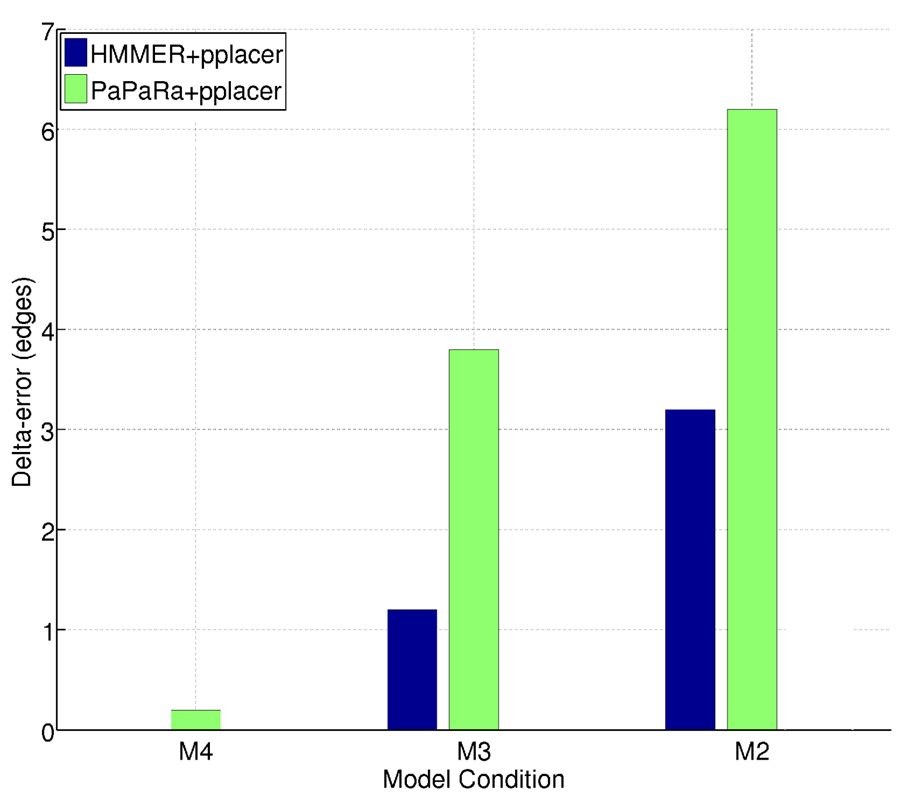
\includegraphics[width=0.80\textwidth]{sepp/hmmer_papara}}
% \caption[Comparison of HMMALIGN+pplacer and PaPaRa+pplacer.]{Comparison of HMMALIGN+pplacer and PaPaRa+pplacer under 3 different model conditions, ranked in order of increasing rate of evolution.  Thus, M4 is the slowest evolving dataset, and M2 is the fastest evolving dataset.  The number of sequences in the backbone set is 500 for all model conditions.} 
% \label{sepp:initial}
% \end{figure}

% In ~\cite{Liu2009}, Liu et al. developed a new alignment and phylogeny co-estimation technique that showed significantly improved alignment and tree reconstruction accuracy on simulated datasets under high rates of evolution (Fig.~\ref{sepp:sate}).  For model conditions simulated under low rates of evolution, all alignment methods had comparable performances.  As the rates of evolution increased, however, alignment and tree accuracy degraded.  This observation lead to the key insight used within \sate: if the evolutionary distance of the sequences could be constrained, then better alignments could be estimated.  By dividing the sequences into subsets of closely related sequences, the evolutionary diameter of the individual subsets is reduced, and more accurate alignments can be estimated on each subset.  The subsets are created using the phylogeny such that sequences that are more closely related will typically fall into the same subset.  This divide-and-conquer approach serves as the basis of the SEPP algorithm.
% 
% \begin{figure}[htbp]
% \centering
% {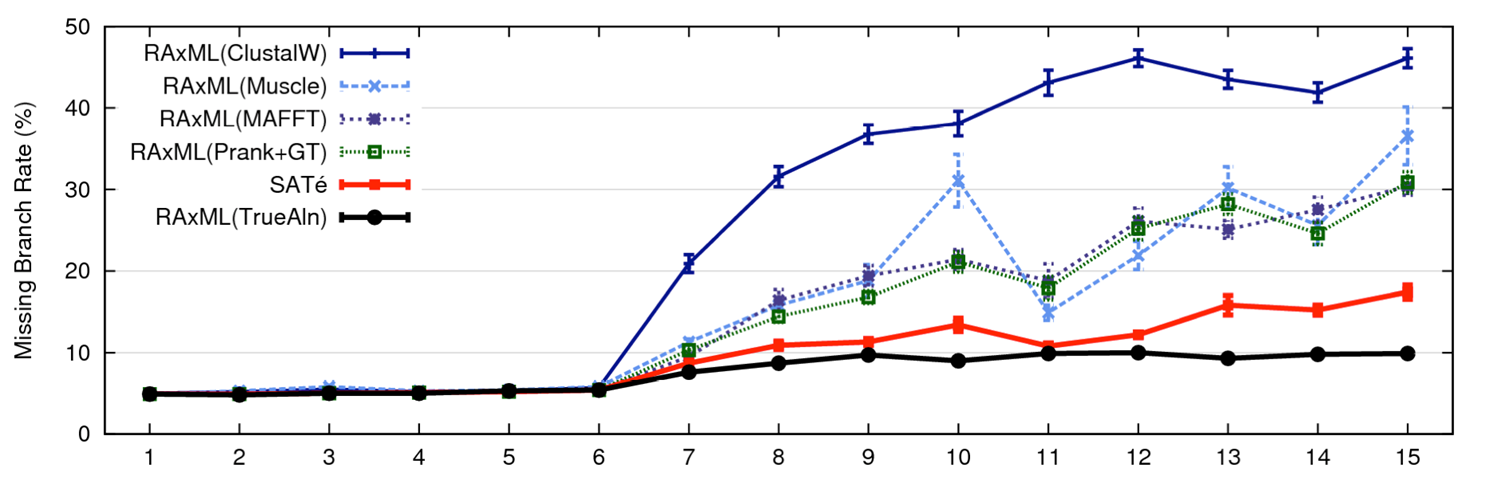
\includegraphics[width=1.00\textwidth]{sepp/sate}}
% \caption[Tree error of RAxML trees estimated on different alignment methods.]{Missing branch rate of RAxML trees estimated on different alignment methods under different model conditions (taken from \cite{Liu2009}).  Each model condition was ranked by difficulty; the higher the model condition number, the more evolution has taken place.} 
% \label{sepp:sate}
% \end{figure}

\section{SEPP algorithm}\label{sepp:algorithm}
SEPP is a meta-method that works with existing
methods for the two steps of phylogenetic placement (computing
the extended alignment, and placing query sequences into
a backbone tree).  SEPP
utilizes upon dataset decomposition technique in
the SAT\'{e}-2 method, which co-estimates sequence alignments and
phylogenies.  This technique takes as input a tree $T$
with leaves labelled by a set $S$ of sequences, a target size $K$,
and it
partitions the set of sequences into smaller subsets, as follows.
SAT\'{e}-2 removes a centroid edge (an edge that
splits the taxon set into two approximately equally sized subsets)
from the input 
tree, thus dividing into two subtrees,
and repeats the process
 until each subset has at most $K$ taxa.
Thus,  the taxa within
any single subset are close together
within the tree and densely sampled within that subset.

The input to SEPP
consists of
\begin{itemize}
\item the backbone tree $T$ and alignment $A$
for the full-length sequences and 
a set of query sequences,
\item
positive integers
\ssa~ and \ssp, with \ssp~$\geq$ \ssa, 
\item a technique for aligning the query sequence
to a multiple sequence alignment of full-length sequences, and
\item
a technique for inserting the query sequence into
a backbone tree, given the extended alignment that
includes the query sequence.
\end{itemize}
The output of SEPP
is the placement of each query sequence into the backbone tree.  The
default methods for SEPP is HMMALIGN for producing the extended alignment
and pplacer for inserting the query sequences into the backbone tree.

%In this study we explore SEPP
%where we use HMMALIGN to produce extended
%alignments and pplacer to insert query sequences into 
%backbone trees.

I now show how SEPP uses the parameters \ssa~ and
\ssp~ to compute the extended alignment and placement of a
set of query sequences
into the tree.
For the sake of simplicity of exposition, I describe this for a single
query sequence.

\begin{itemize}
\item 
SEPP uses the SAT\'{e}-2 decomposition strategy 
to divide the set of taxa in the tree $T$
into disjoint subsets of size at most \ssp.
These subsets are called the ``taxon-insertion-subsets."
\item
SEPP further divides each taxon-insertion subset 
into smaller subsets of size \ssa.
These subsets are the ``alignment--subsets".
Thus, each  alignment-subset is a subset of 
exactly one taxon-insertion-subset.
\item SEPP computes the HMM profile using HMMER for each of the alignment-subsets,
and SEPP finds the alignment-subset that the query sequence $s$ has the best
match to.  HMMALIGN is used to produce an alignment of
$s$ to the backbone alignment on the alignment-subset,
and then that alignment is used to produce the extended alignment for
$S \cup \{s\}$. 
\item 
SEPP finds the taxon-insertion-subset that contains
the selected alignment-subset, and
pplacer is used to insert 
the query sequence $s$ into the 
subtree of the backbone tree induced by the taxon-insertion-subset.
Finally, the location of $s$ in the subtree is used to insert
$s$ into the backbone tree on the entire set of taxa.
\end{itemize}
Thus, the two  parameters \ssa~ and \ssp~ control the
behavior of SEPP.
%We let  \ssa~ range from 10 to 250
%for the simulated datasets and from 10 to 2500 for the biological
%dataset.  We let \ssp~ range from 10 to 500 for the simulated
%datasets and from 100 to 13,822 for the biological dataset.

\section{Performance evaluation}\label{sepp:evaluation}

In order to evaluate SEPP's performance, I compared SEPP 
versus HMMALIGN+pplacer and PaPaRa+pplacer on both 
empirical and simulated datasets.  

I studied performance of these phylogenetic
placement methods on 61 sequence datasets\footnote{All
datasets used in this study are available at 
http://www.cs.utexas.edu/~phylo/datasets.}.
I included 20 simulated 1000-taxon datasets 
that have evolved with substitutions and indels 
from each of three different model
conditions (M2, M3, and M4),
each with the ``medium" gap length distribution
(see Liu et al.\cite{Liu2009} for these data). 
The three model conditions are chosen such
that one dataset is hard, one is moderate, and one is easy.
Because these are simulated datasets,
the true alignment and true tree are known for each datasets. 

I also used
a large bacterial dataset, 16S.B.ALL, with 27,643 16S rRNA sequences, 
originally taken from the Gutell Comparative
Ribosomonal Website (CRW)\cite{Cannone2002}, and also studied by
Liu et al.\cite{Liu2011}.
This dataset has
a curated alignment based upon confirmed secondary (and higher-order)
structures, which are highly reliable.
I use a ML bootstrap tree as the curated
tree for this dataset, retaining only those branches with bootstrap
support above 75\%\cite{Liu2011}. 
Thus, the 16S.B.ALL dataset has a curated tree and alignment as well.

Each dataset was randomly divided into two subsets of equal size,
with one subset ($S$) used to define the backbone alignment and tree,
and the other subset ($R$) used to produce the query sequences.
These query sequences are created by taking substrings of 
normally-distributed lengths (from two distributions, described below), and
with the start positions chosen uniformly at random.

Two categories of reads are generated for each sequence in the M2, M3, and M4
datasets:
``long'' reads, with a mean length of 250 and a standard deviation of 60, 
and ``short'' reads, with a mean length of 100 and a standard deviation of 20.
A total of 10 fragmentary sequences are generated for each sequence,
with half long and half short.  Since
these datasets each include 500 reference and 500 non-reference sequences, 
this process yields 2500 short  and 2500 long reads per dataset.
In summary, each M2, M3, and M4 dataset has a reference tree and alignment 
with 500 taxa and a total of 5000 fragmentary sequences, of which half are
``short" and half are ``long".

For the 16S.B.ALL biological dataset, I create two categories of reads,
with length distributions identical to those of simulated datasets. 
This dataset contains 27,643 taxa, of which I use
13,822 sequences for the backbone tree, leaving me with 13,820 sequences
for creating fragmentary reads. 
For each of these
13,821 sequences, I generated one fragmentary sequence, 
randomly choosing between the long and
short distributions.  Thus, for 
this dataset the backbone tree and alignment has 13,822 taxa, and
there are 13,821 fragmentary sequences.

The sequences in $S$ are used to create two backbone alignments and
trees, as follows.
For sets $S$ that are produced by
simulating sequence evolution,  I have the true alignment and
the true tree.
I restrict each of these (which have 1000 taxa) to the subset of 500
full-length sequences, and then run RAxML
on the resultant tree/alignment pair in order to
optimize the branch lengths and GTR+Gamma parameters.   
This produces the first alignment/tree backbone.
The second backbone alignment/tree pair is produced by running
SAT\'{e} on the set of full-length sequences.
%This analysis produces a tree topology and alignment with 
%GTR+Gamma model parameters optimized
%on this tree/alignment pair.

For the 16S.B.ALL dataset, I use the curated alignment for the
dataset and run RAxML on the alignment to produce a binary
tree.  I then 
restrict the tree to the subset of 13,822 sequences, and 
optimize the branch lengths and GTR+Gamma parameters on the tree
using RAxML.
This produces the first
backbone alignment/tree pair. I use
SAT\'{e} on the subset of 13,822 full-length sequences
to produce the second.
% (with RAxML used to optimize
%the model parameters on the output tree/alignment pair).

I used SAT\'{e} to produce these estimated alignment/tree pairs
because SAT\'{e} produces
more accurate alignments and trees than any two-phase method
(where an alignment is first estimated and then a tree
computed on that alignment)
for these datasets\cite{Liu2011}.
I used SAT\'{e}-2, the new algorithm design for SAT\'{e}, for
these analyses; this produces an alignment and an ML
tree on the alignment estimated using RAxML.
For the 16S.B.ALL dataset, I used FastTree\cite{Price2010}
within SAT\'{e}-2 in each iteration, and finished with
RAxML in order to produce optimized GTR+Gamma parameters on
the final tree.

I classify each query sequence
for its likely difficulty in phylogenetic placement as follows.
I use \hmmer to produce a
HMM profile for the reference alignment, and then to classify the 
query sequences with respect to the HMM profile.
The fragmentary reads are classified as easy to align (``easy") if the obtained
E-value is less than $10^{-5}$, and as ``hard'' otherwise.
Among the hard
reads, there are some reads for which HMMER does not report 
any E-value due to default filtering settings of HMMER. 
I classify such reads as ``very hard" reads.
In earlier phylogenetic placement studies, the hard fragments are
excluded~\cite{Matsen2010}; however,  my study does not 
automatically
eliminate hard fragments.
Many very hard reads are able to be placed by
SEPP, because the reads will receive
E-values with respect to the
smaller alignment subsets.  
Those that fail to be placed at all by SEPP are 
removed from the experimental study; this
process removes 9 from all the
simulated datasets together and 5 from the biological
dataset.

\begin{table}[htbp]
\begin{small} \centering
 \caption{Dataset statistics: 
I present statistics for the true alignments for
the simulated datasets (M2, M3, M4) and
statistics for the curated alignment
on the biological dataset, 16S.B.ALL.
However, a small number of query sequences is
deleted from some of the runs.
}
\begin{center}
\begin{tabular}{clrrllc}
\hline
\hline
Dataset & Type& Size & Num generated     	& Avg 		& Max&  \% gap\\
 	& 	&backbone & query seqs 	& p-dist 	& p-dist & \\\hline
M2 		& sim& 500 & 5000& 0.68 & 0.76 & 67\\\hline
M3 		& sim& 500 & 5000& 0.66 & 0.74 & 53\\\hline
M4 		& sim& 500 & 5000& 0.50 & 0.60 & 51\\\hline
16S.B.ALL 	& emp& 13,822& 13,820 & 0.21 & 0.52 & 74\\
\hline
\end{tabular}
\end{center}
 \label{tab:datasets}\end{small}
\end{table}

Table~\ref{tab:datasets} shows various statistics for the 
true or curated alignment of the datasets included in
our study. The p-distance is the
fraction of sites within an alignment in which two sequences are
different and ``\% gaps" is the percentage of gaps within the alignment.
The empirical statistics show that the datasets vary substantially
in terms of evolutionary distances, with datasets from
model M2 having the largest evolutionary 
distances and 16S.B.ALL having the smallest.

\section{Measurements}
I measure placement accuracy (averaged over
all the query sequences),  running time,
and peak memory usage, for each method on each dataset.
For the simulated datasets I report averages for these
measurements over the 20 replicates in each model
condition.  

% \subsection{Placement accuracy}
% For the most likely
% placement\footnote{Multiple possible placements for
% each read, along with the likelihood of each placement,
% are also provided by pplacer.} of each fragmentary
% read, I first calculate the number of missing branches compared to the 
% reference tree. 
% This number in isolation is hard to interpret, for at least two reasons.
% In the case where \sate~alignment/tree is the input, the backbone tree itself
% contains error. The error of the initial backbone tree is a lower bound on the
% tree error after placement of reads (in fact it is a rather liberal lower bound,
% as the optimal placement of fragments can still have errors higher than the
% initial tree).
% In the case where true or curated alignment/tree is 
% the input, the initial tree has no
% error, but I can still establish useful lower bounds of the tree error. 
% This can be done by using the reference alignment of query sequences 
% to be the backbone alignment as input to the \pplacer. 
% The resulting placement of query sequences
% is the best one can realistically hope for.
% %Siavash - note that randomness is also an explanation for
% %having delta error below 0.  This makes me wonder if we might not just
% %show the delta as the additional error over the error before insertion.
% %ALSO: need to comment on difference between error to true tree and
% %error to ML on true or curated alignment.
% %and perhaps we should show the actual error instead of delta error.

% To account for the lower bounds described above,
% I also define and report 
% the ``delta error" for each technique,  as follows.
% For each read $s$ placed on the \sate~backbone tree, 
% I report the difference between
% the number of missing branches of the initial 
% backbone tree 
% and the number of missing branches after placement of $s$.
% When the backbone tree is 
% the reference (true or curated) tree, 
% I report the
% difference between the number of missing branches of the tree produced by
% placement of $s$ according to the 
% reference alignment of $s$ to $S$ and 
% the number of missing branches
% of the tree after placement of $s$.
% In all cases, 
% the number of missing branches in each tree is defined with
% respect to the reference tree for the taxa in the given tree.
% Thus, the number of missing branches in the backbone trees is
% defined by the reference tree on the set $S$ of backbone taxa, and the
% number of missing branches in the tree produced by placing the
% query sequence into the backbone tree is defined by the
% reference tree on the set $S \cup \{s\}$.


% Note that in the case where the backbone tree is the reference tree, 
% the number of missing branches is
% equal to the node distance between the correct placement of reads and
% actual placements, the error used in the literature\cite{Berger2011,Matsen2010,Berger2011a}. 
% However, this edge distance is not as meaningful as the 
% number of missing branches with respect to either the true or
% curated tree, since estimated trees will generally have error.

\subsection{ Computational aspects}
I report the running times and peak memory usage, each measured
separately for the computation of
extended alignments and placement of query sequences.
These reported values are for 
alignment and placement of all query sequences in each set.
Since some query sequences are deleted from the study as
they cannot be placed, the total number of
query sequences is slightly smaller than the number
generated.
Thus, results for each simulated model condition
are for 99997-100000 query sequences (20 replicas, each with 5000 query sequences),
results for 16S.B.ALL are for 13,819-13,821 query sequences.
Due to memory requirements of PaPaRa and pplacer, 16S.B.ALL experiments are
run on a Linux machine with 16 cores and 256GB of main memory. The results
for simulated datasets are obtained on a heterogeneous condor
cluster.
\section{Results}\label{sepp:results}
\subsection{Algorithm design experiments}

\begin{figure}[htbp]
  \centering
  \subfloat[16S.B.ALL, Curated backbone]
{\label{fig:stt}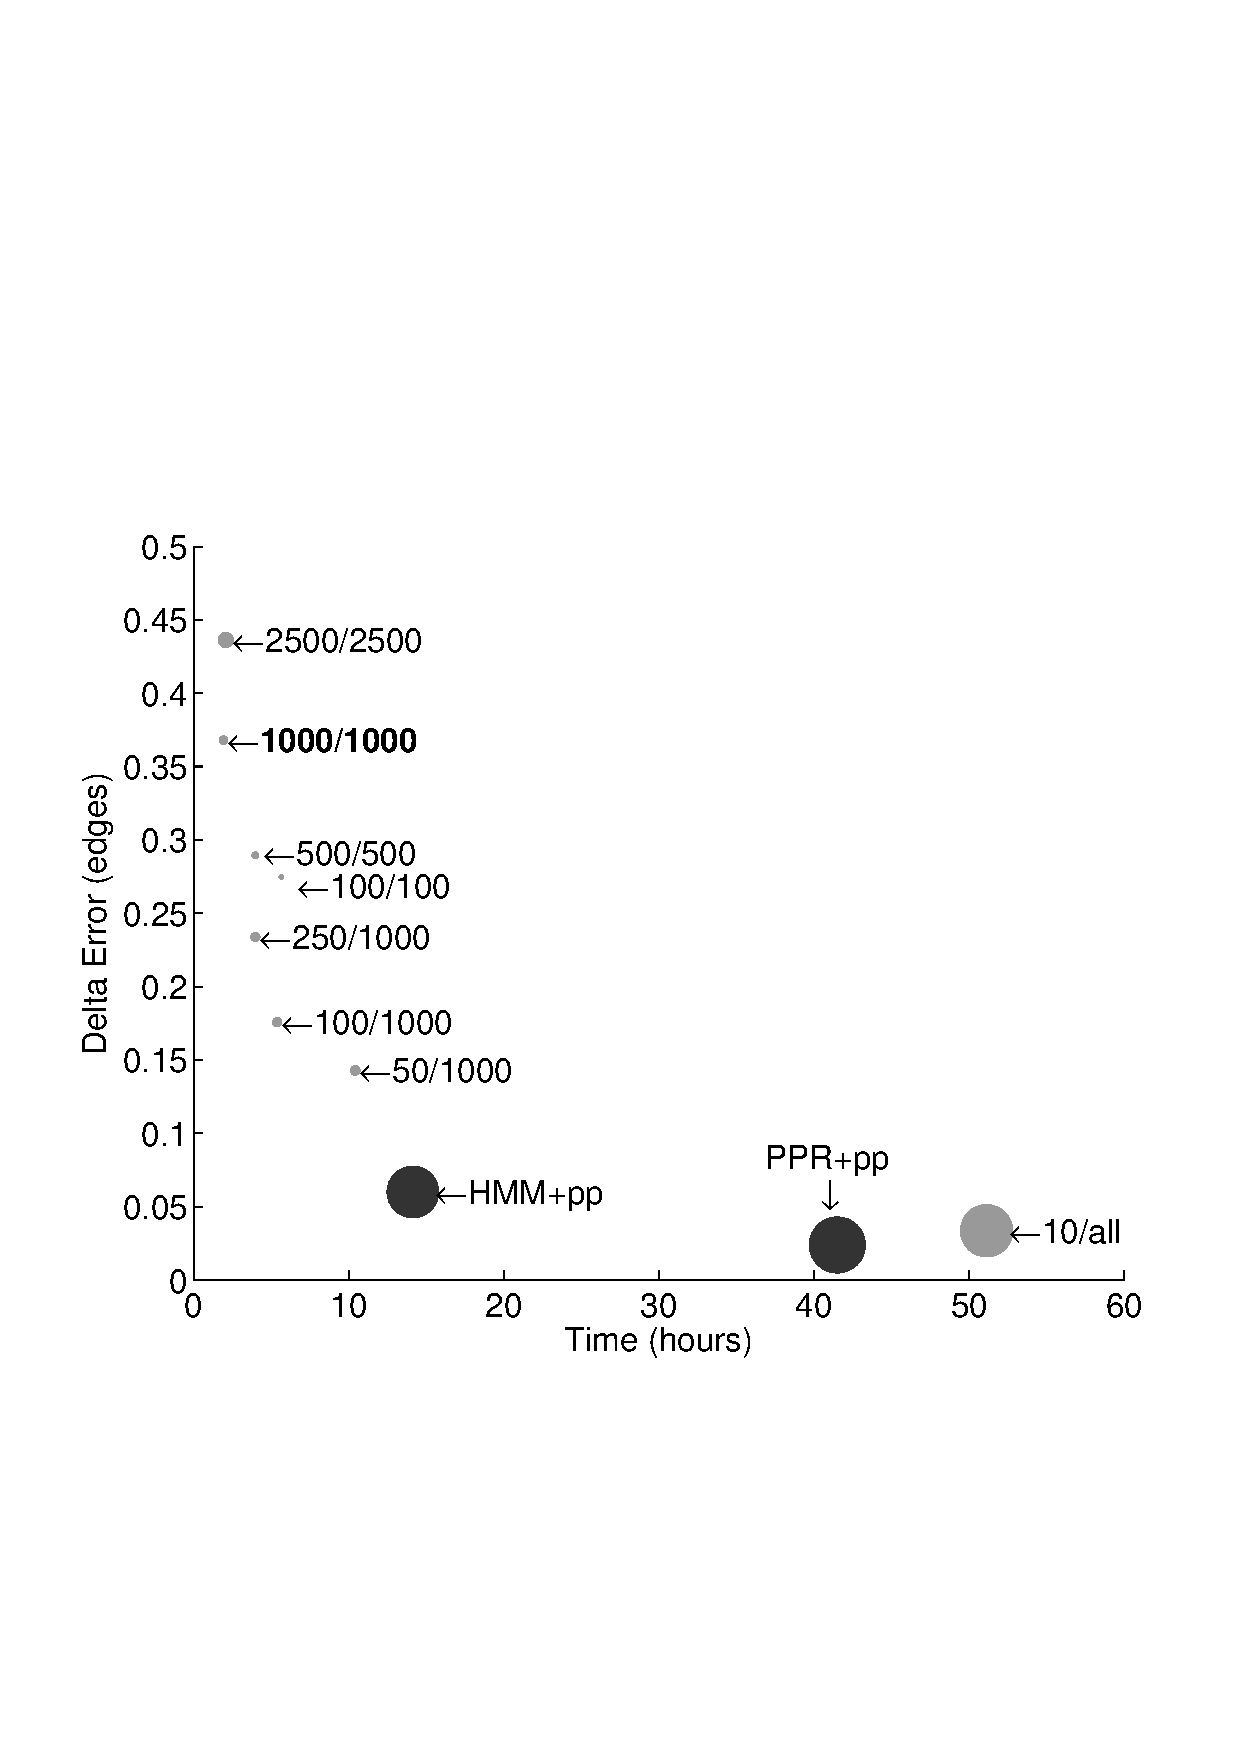
\includegraphics[width=0.70\textwidth]{sepp/scatter-bio-true}}
  \subfloat[16S.B.ALL, \sate~backbone]
{\label{fig:sts}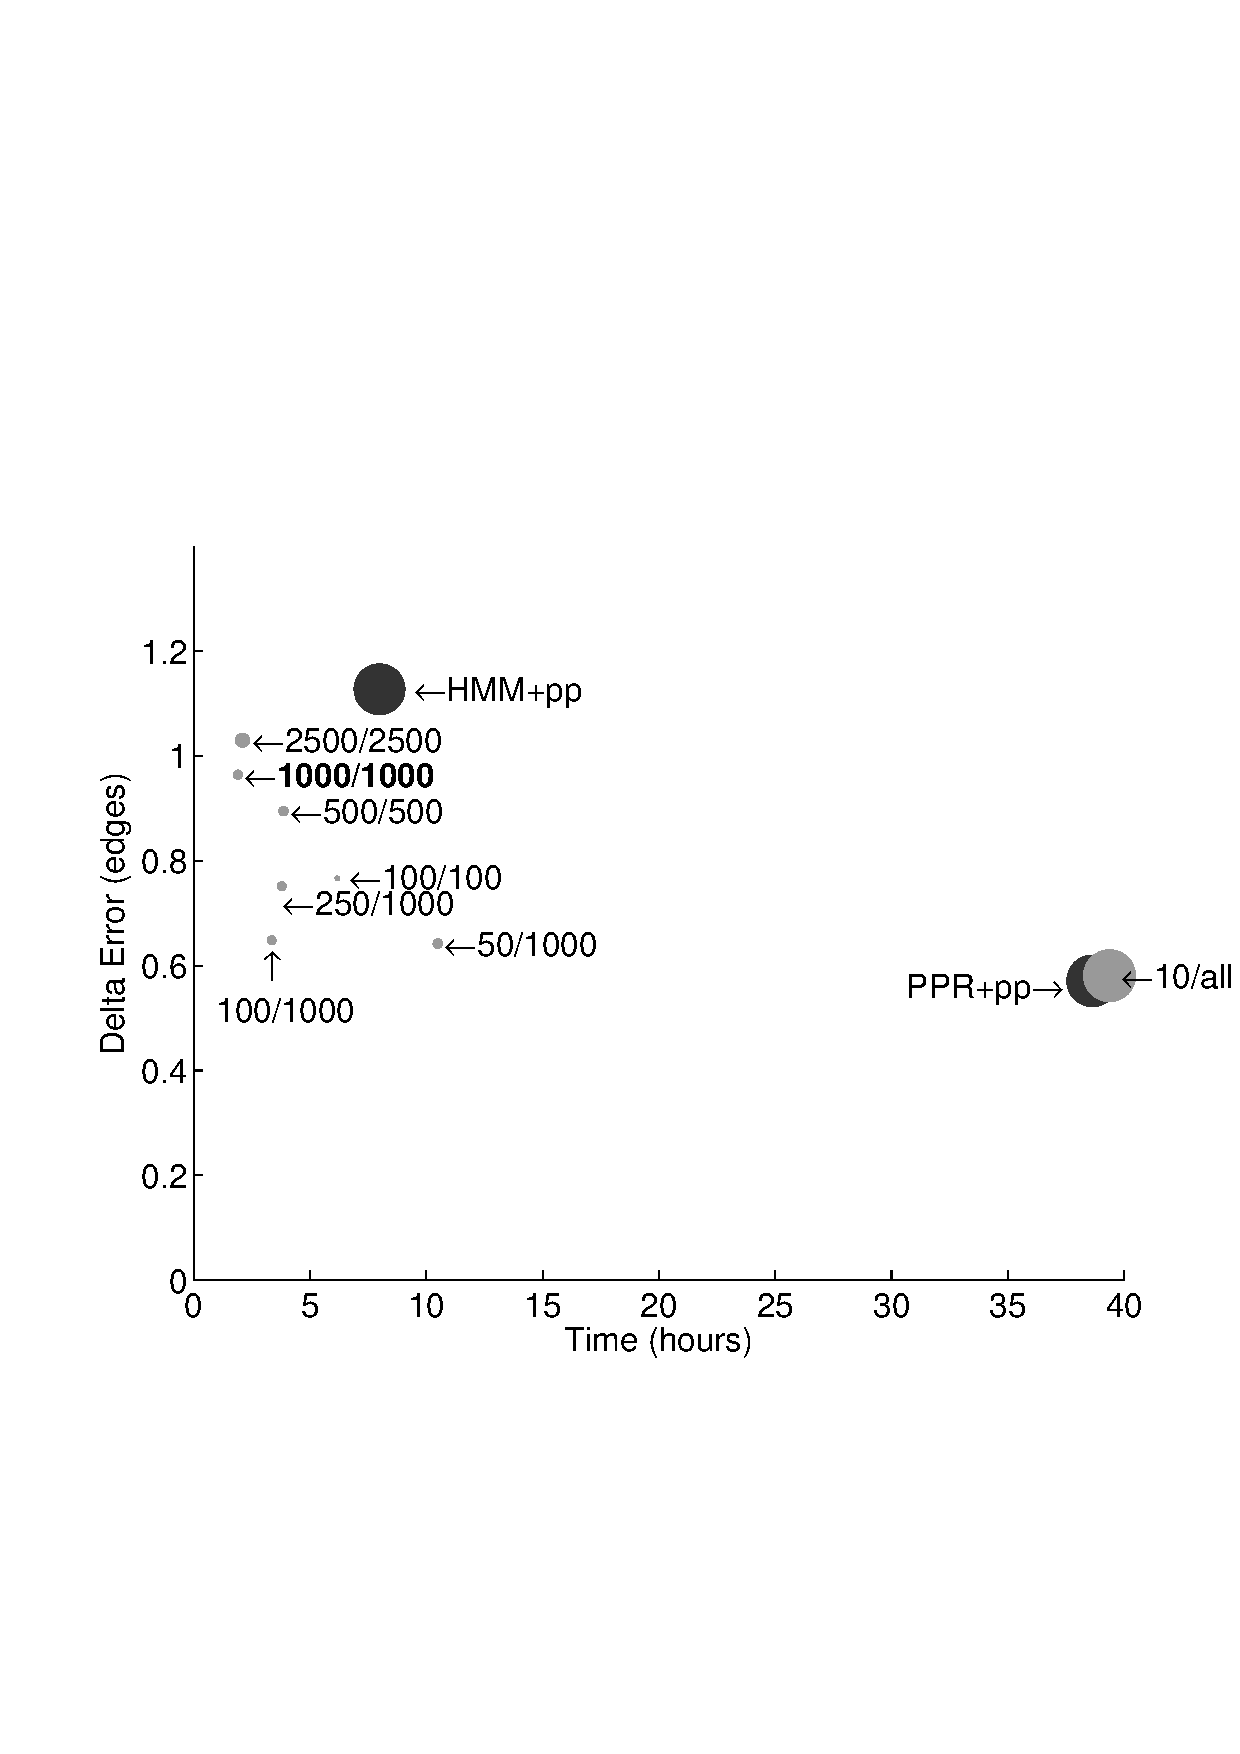
\includegraphics[width=0.70\textwidth]{sepp/scatter-bio-sate}}
\\
  % \subfloat[M2, \sate~backbone]
% {\label{fig:smt}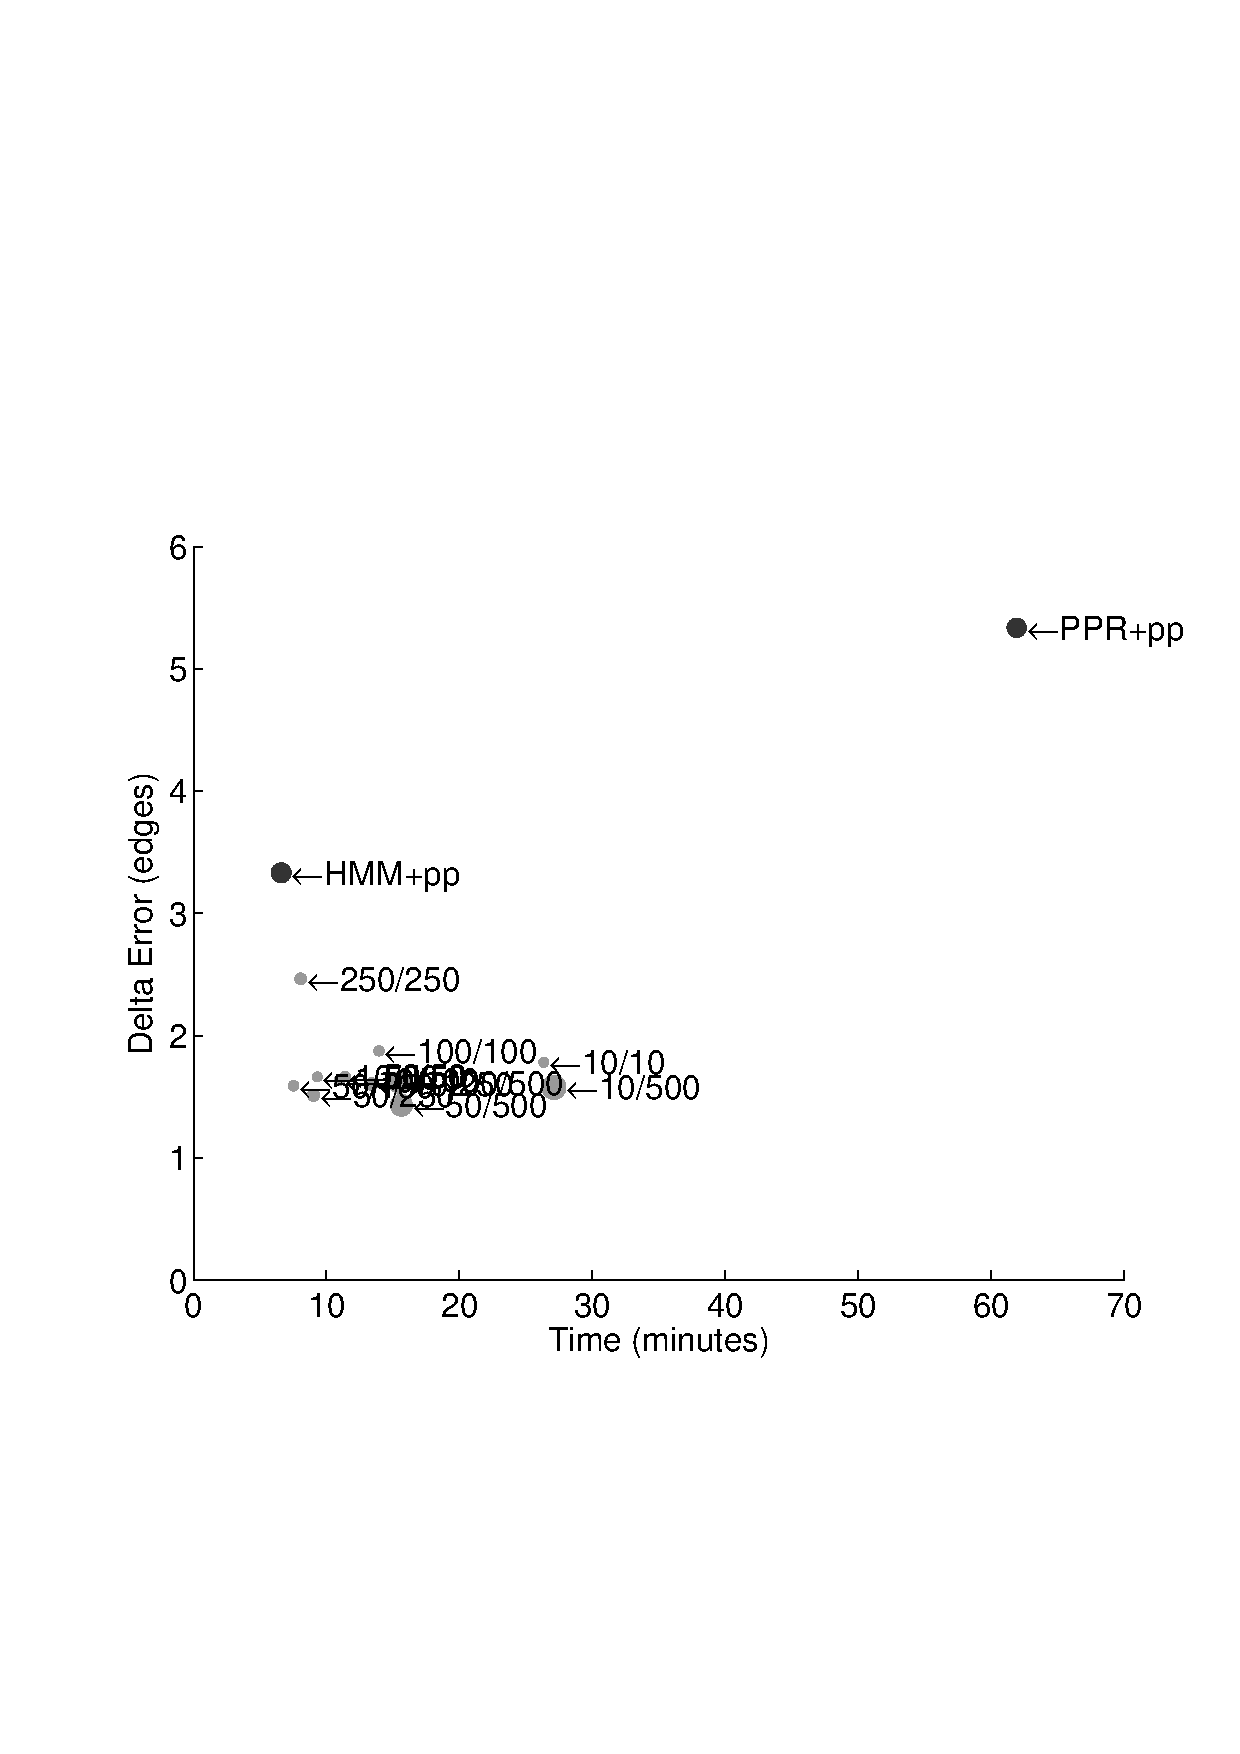
\includegraphics[width=0.5\textwidth]{sepp/scatter-sim-sate}}
  % \subfloat[M2, \sate~backbone - most accurate settings]
% {\label{fig:sms}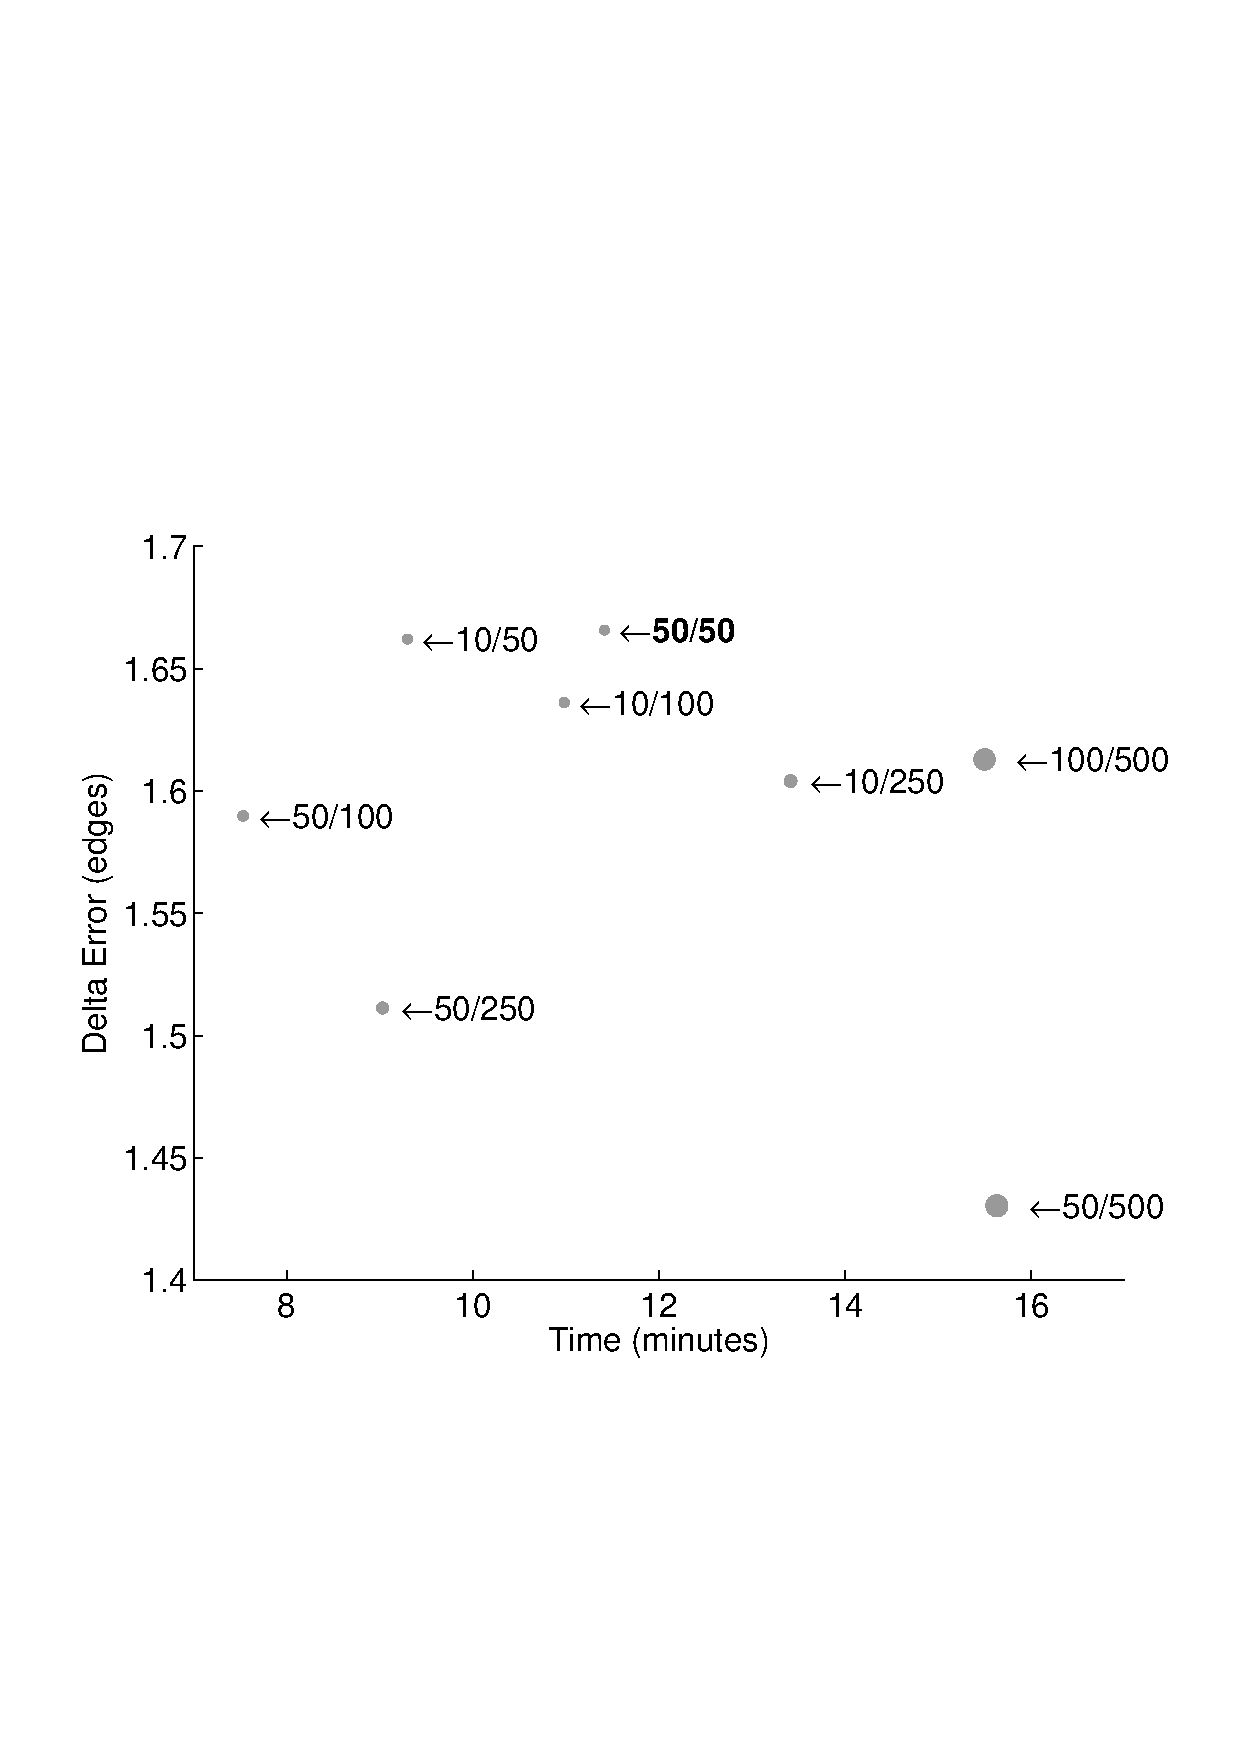
\includegraphics[width=0.5\textwidth]{sepp/scatter-sim-sate-blowup}}
  \caption{Scatter plot of delta error (x) versus time (y) versus memory
(circle diameters). The symbol ``x/y" refers to SEPP(x,y). The default
setting is 1000/1000 for 16S.B.ALL; these points
are bold-faced. Note that the default setting for SEPP is
far from optimal, with other settings providing
better accuracy (and in some cases also better speed).} 
  \label{fig:design-bio}
\end{figure}

\begin{figure}[htbp]
  \centering
  % \subfloat[16S.B.ALL, Curated backbone]
% {\label{fig:stt}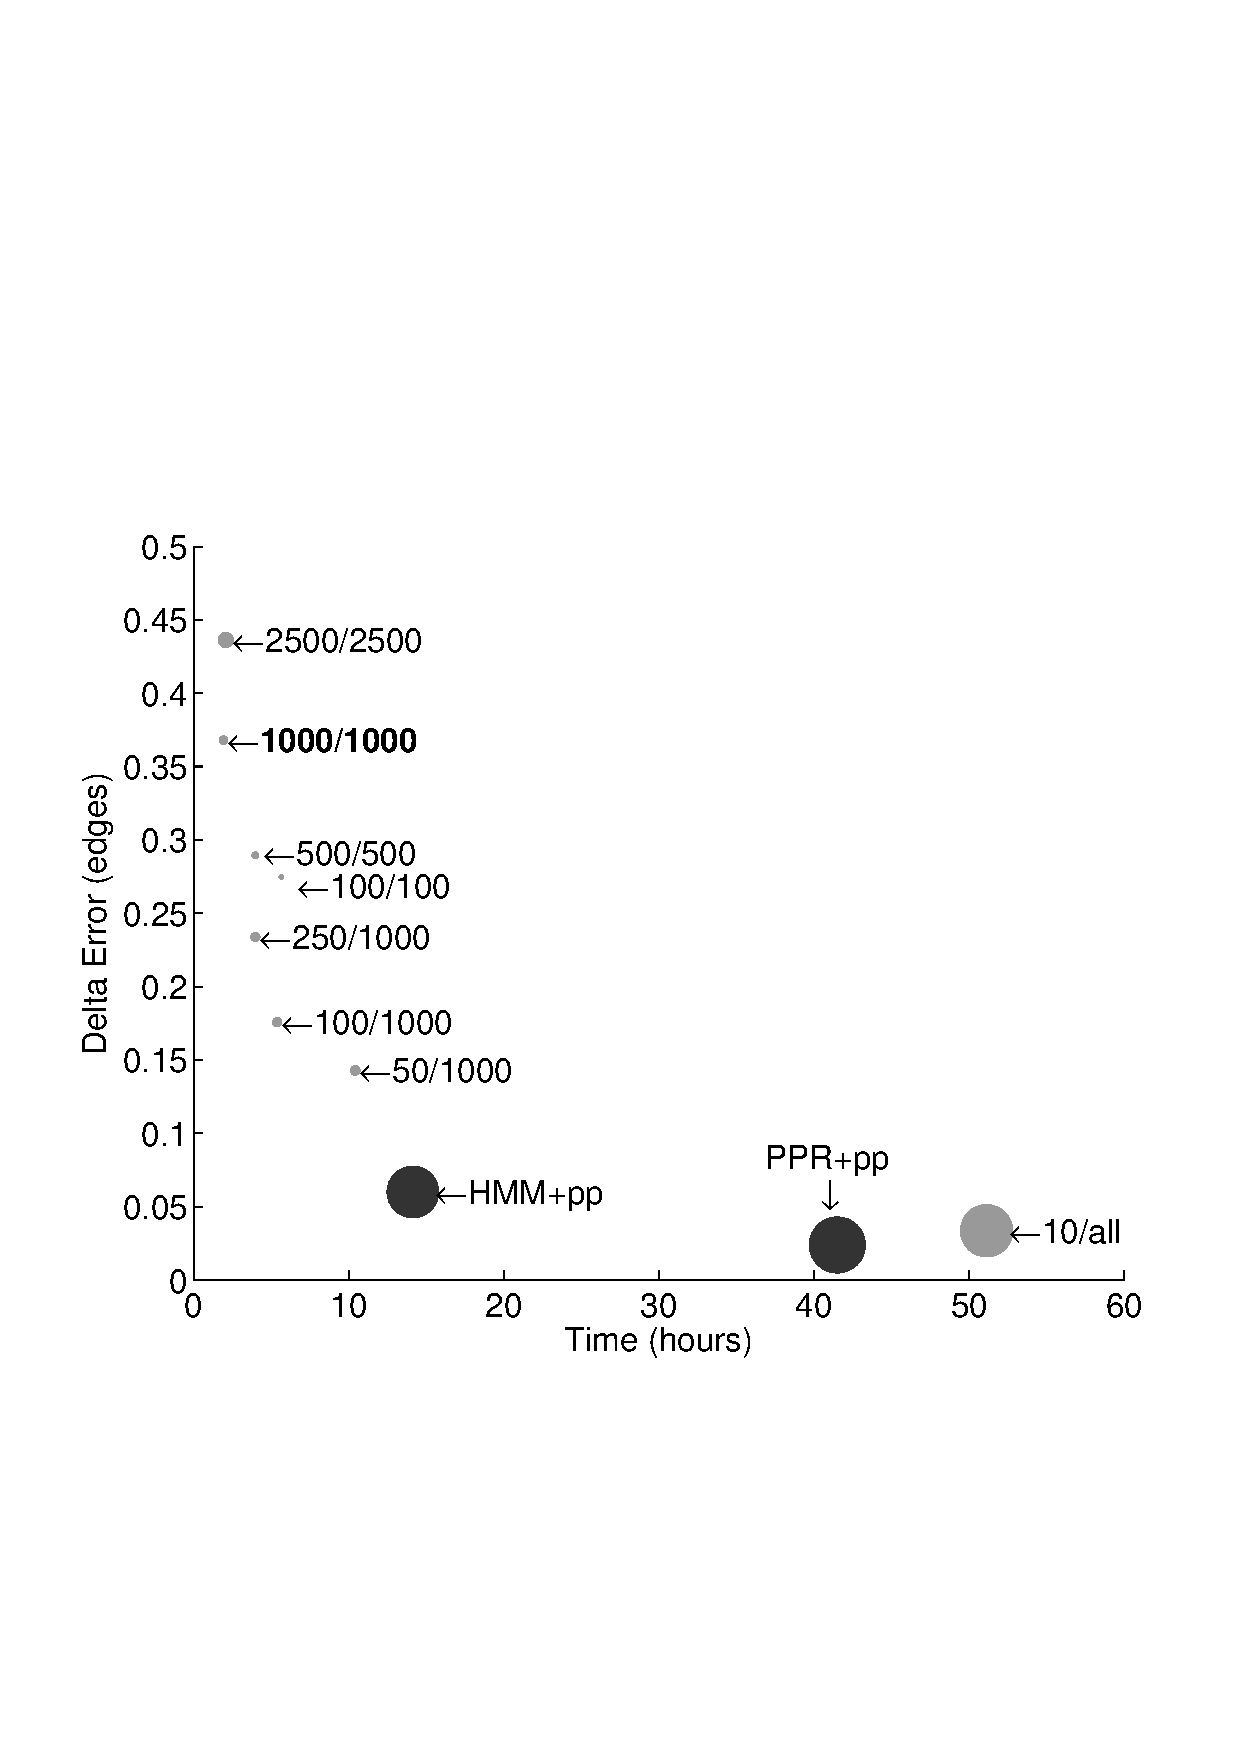
\includegraphics[width=0.5\textwidth]{sepp/scatter-bio-true}}
  % \subfloat[16S.B.ALL, \sate~backbone]
% {\label{fig:sts}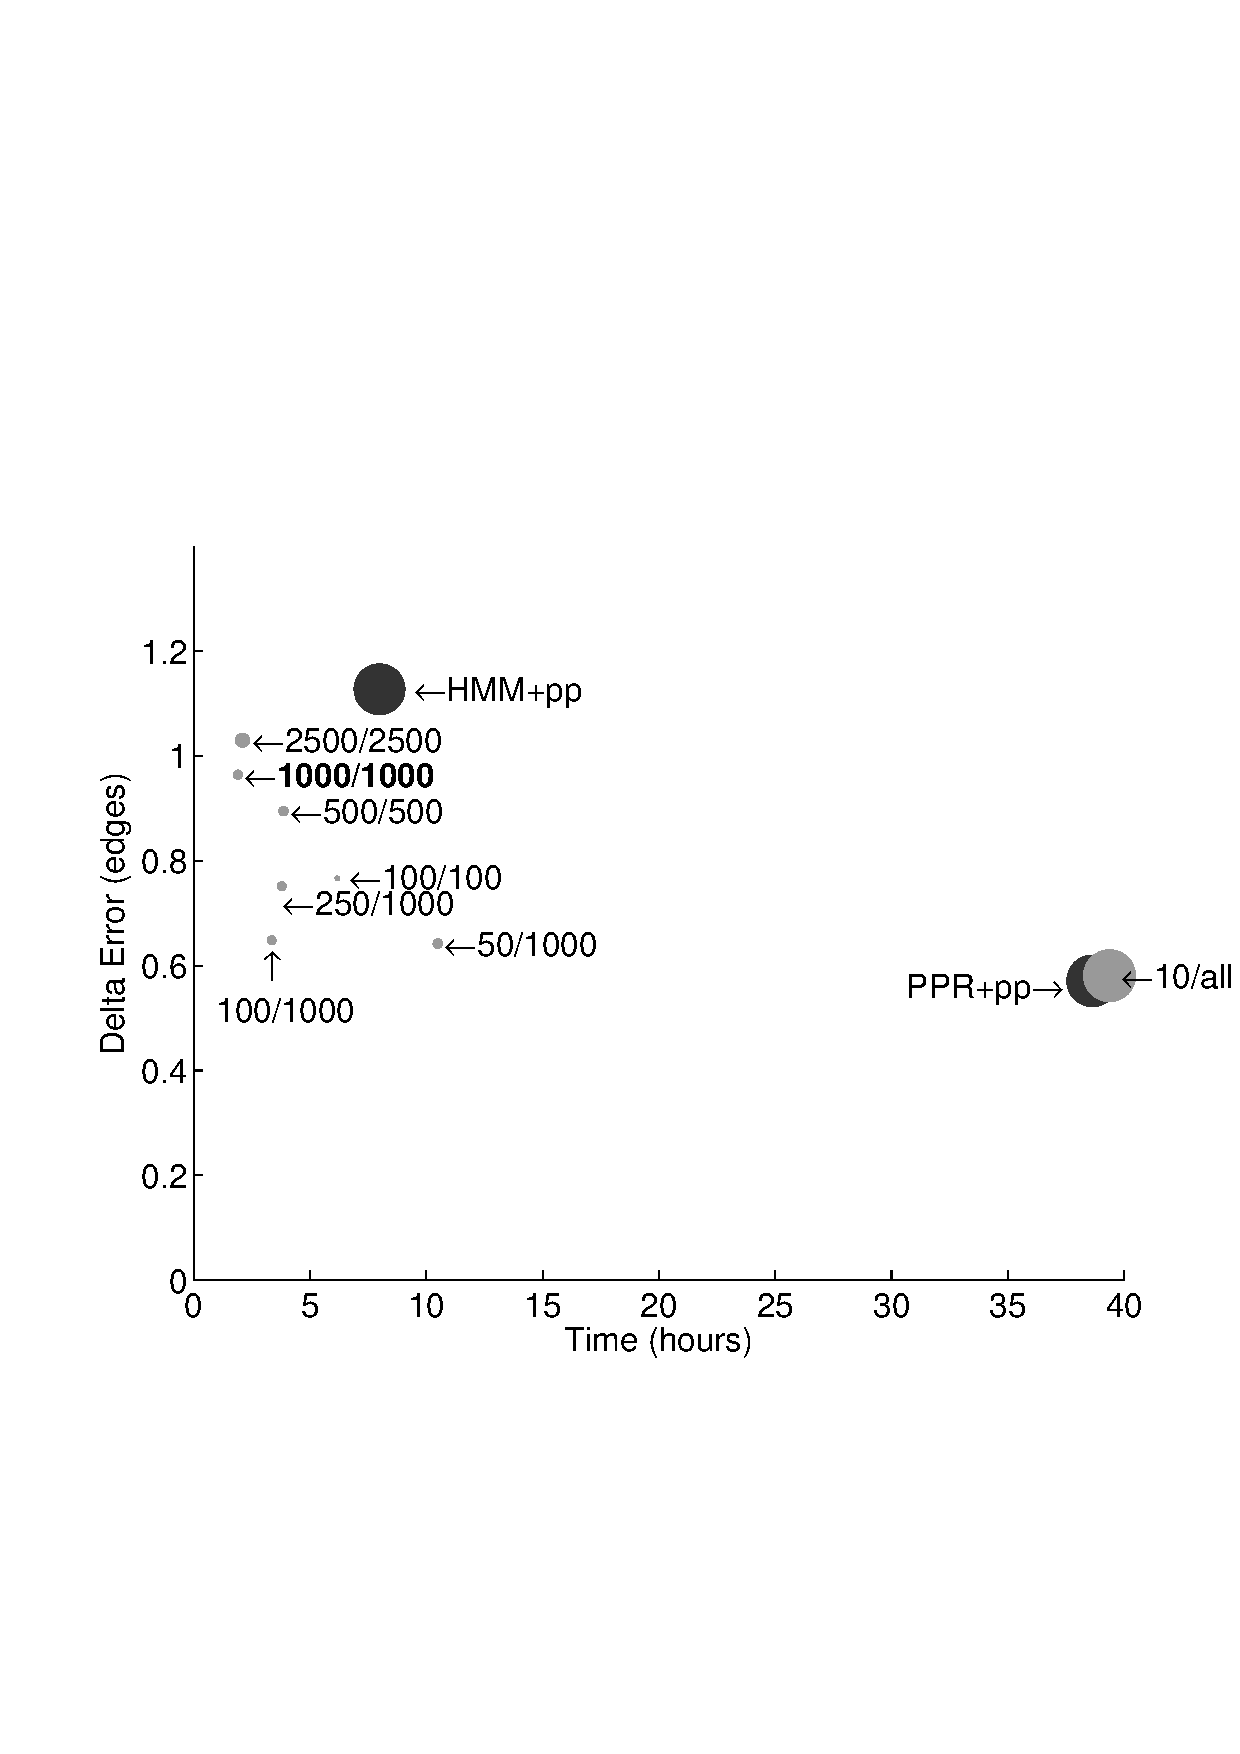
\includegraphics[width=0.5\textwidth]{sepp/scatter-bio-sate}}
% \\
  \subfloat[M2, \sate~backbone]
{\label{fig:smt}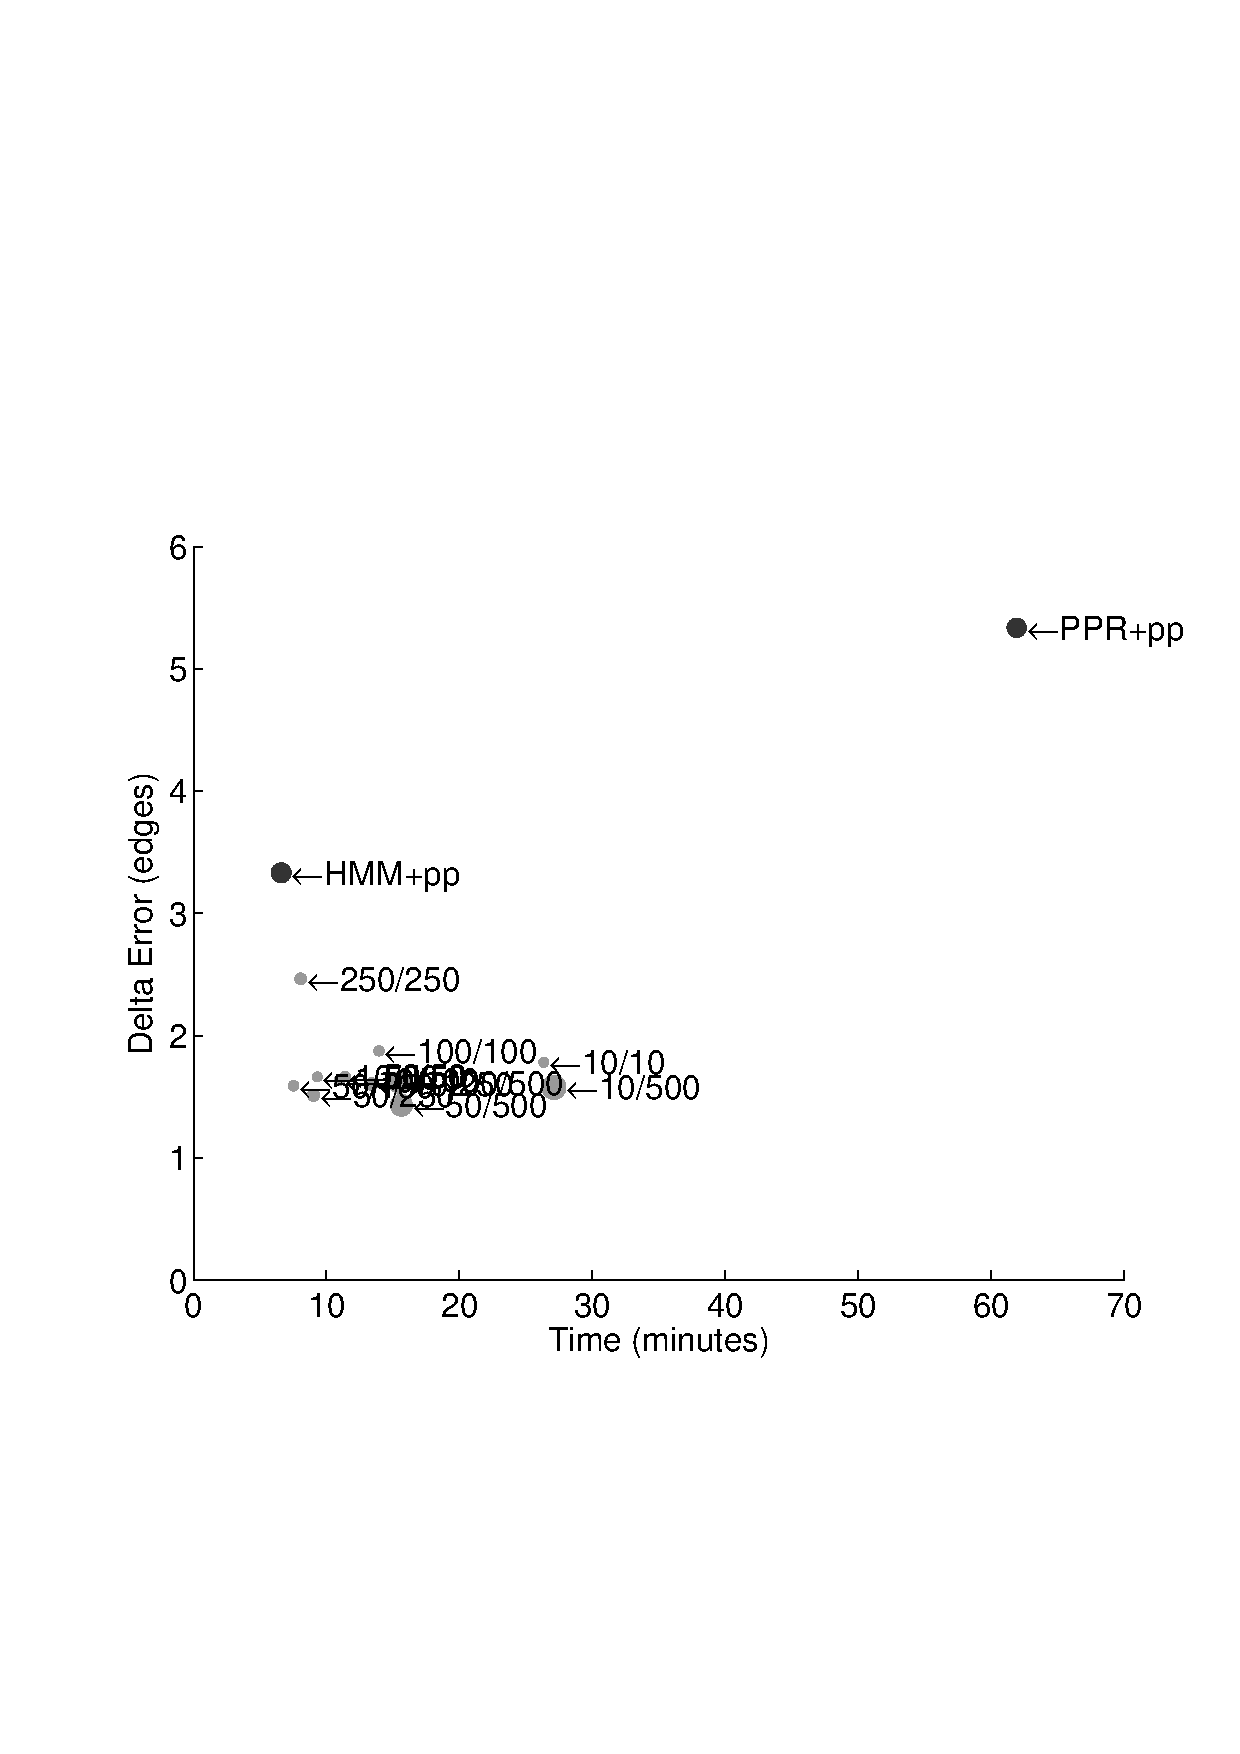
\includegraphics[width=0.70\textwidth]{sepp/scatter-sim-sate}}
  \subfloat[M2, \sate~backbone - most accurate settings]
{\label{fig:sms}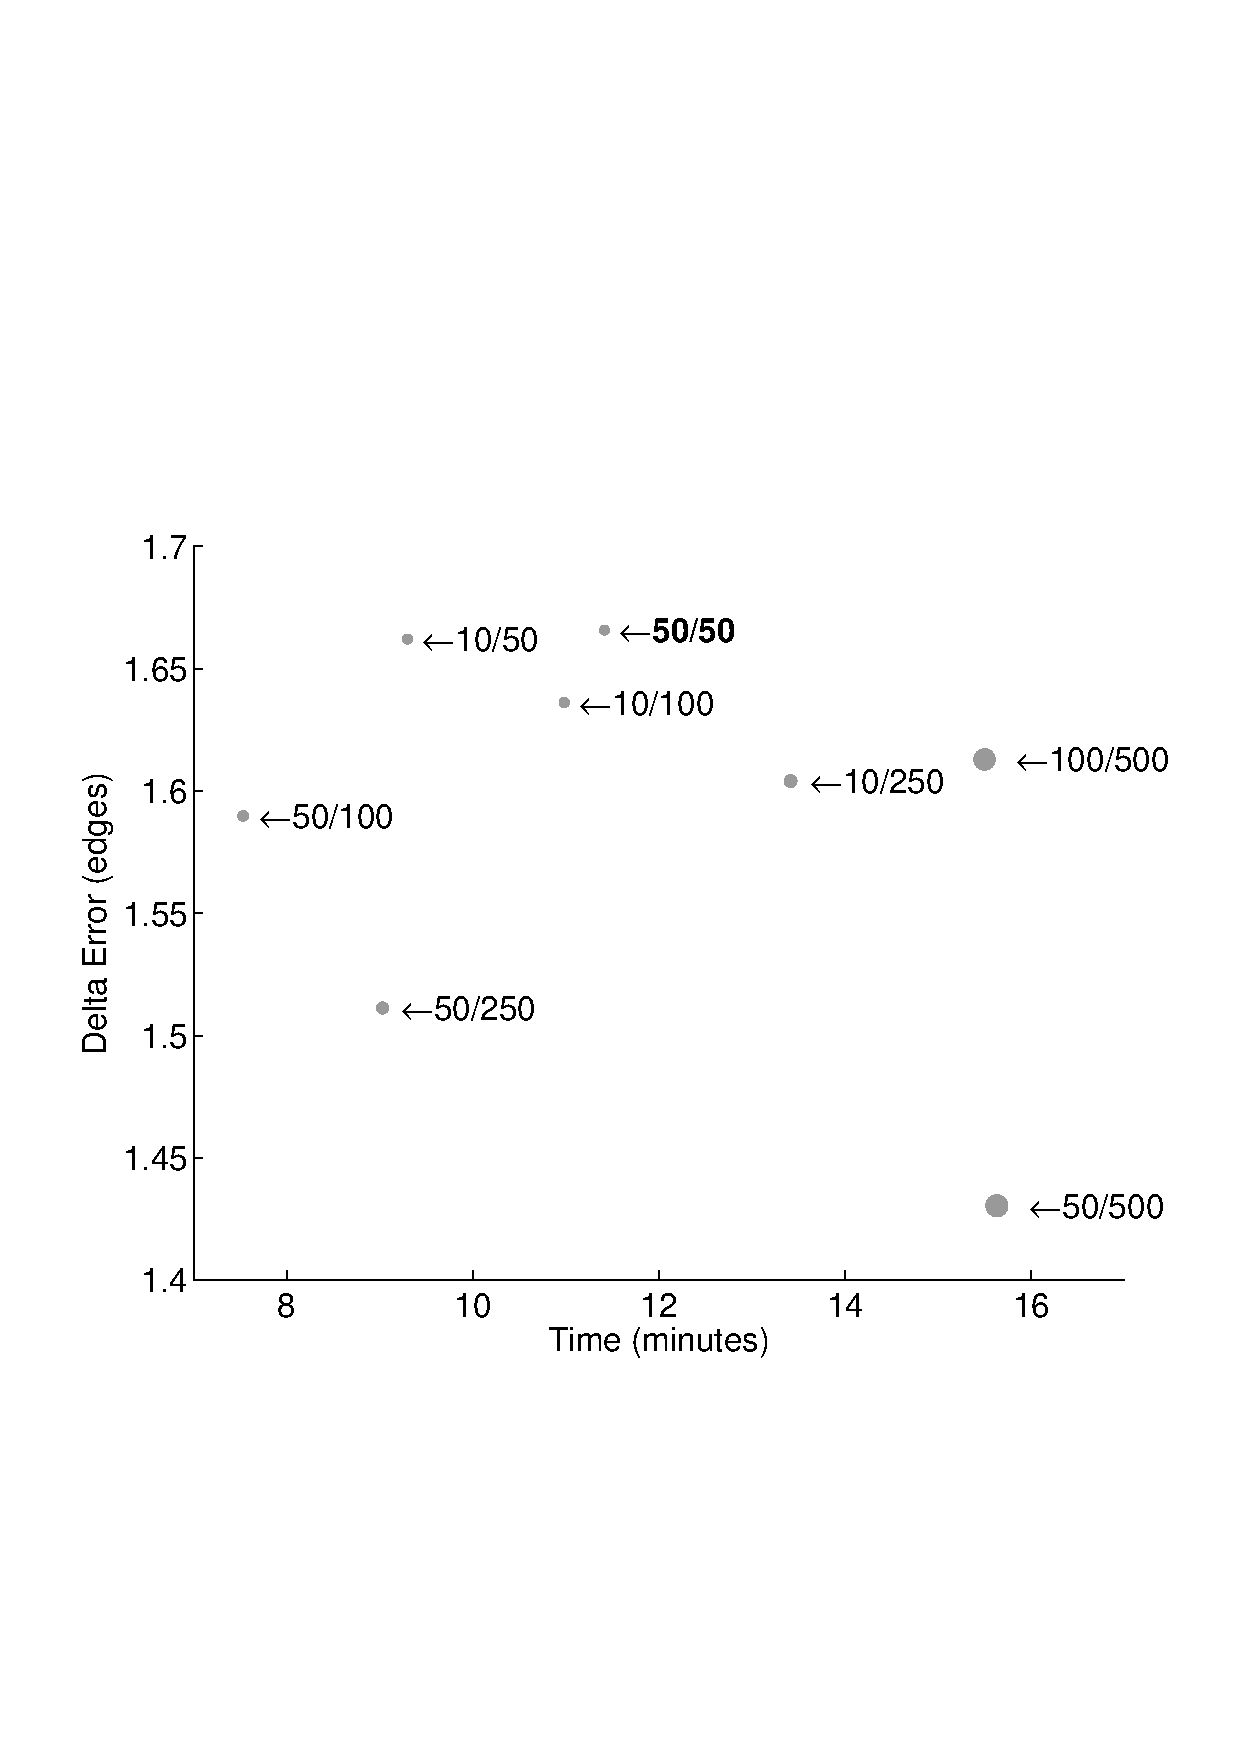
\includegraphics[width=0.70\textwidth]{sepp/scatter-sim-sate-blowup}}
  \caption{Scatter plot of delta error (x) versus time (y) versus memory
(circle diameters). The symbol ``x/y" refers to SEPP(x,y). The default
setting is 50/50 for M2; these points
are bold-faced. Note that the default setting for SEPP is
far from optimal, with other settings providing
better accuracy (and in some cases also better speed).} 
  \label{fig:design-sim}
\end{figure}


Figures \ref{fig:design-bio} and \ref{fig:design-sim} show results 
where I vary the two algorithmic parameters
\ssa~ and \ssp.
Note that decreasing \ssa~ to 50 (and sometimes to 10) 
and increasing \ssp~ tends to
improve the placement accuracy, but at a running time cost.
Also, bigger improvements in accuracy are obtained by decreasing
\ssa~ than by increasing \ssp.  However, for most conditions,
there is a wide range of parameter settings in which the
differences in placement error are quite
small (often less than half an edge), and
within this collection there can be significant differences in running
time.

To set the default parameters, I sought a setting that
worked reasonably well with respect to both
running time and placement accuracy. 
Setting \ssa=\ssp=1000 for the 16S.B.ALL
datasets and \ssa=\ssp=50 for the
simulated datasets  produced good results.  These
settings correspond to setting the subset sizes to about
10\% of the number of taxa in the
backbone tree.
Note, however, that setting \ssa=\ssp=50 is by no means optimal for the M2
model condition (four other settings, with \ssa~at most 50,
have less error and complete faster).
Similarly, setting \ssa=\ssp=1000 is the fastest for the
16S.B.ALL datasets, but more accurate
results can be obtained with other settings (each
with \ssa~below 1000)
for a running time cost.

\vspace{.1in}
\subsection{Comparisons using the default setting for SEPP}

I present results for PaPaRa+pplacer, HMMALIGN+pplacer, and
the default setting for SEPP where we set
\ssa= \ssp~to approximately 
10\% of the number of taxa in the backbone tree. This yields
parameters 50/50 for the simulated datasets (backbone trees have 500
taxa) and 1000/1000 for the 16S.B.ALL dataset (backbone
trees have 13,822 taxa).

\begin{figure}[htbp]
  \centering

%  \subfloat[\sate~backbone]
{\label{fig:sts}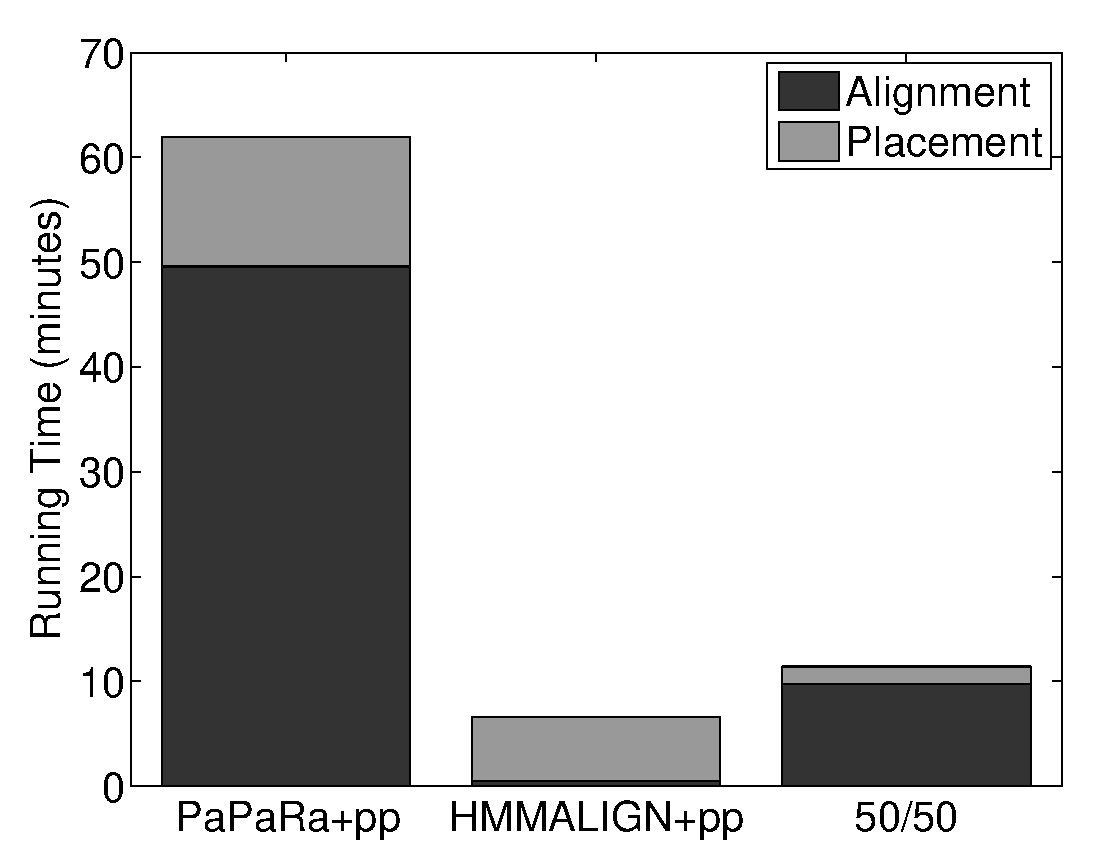
\includegraphics[width=0.35\textwidth]{sepp/M2-time-sate}}
%  \subfloat[True backbone] 
{\label{fig:stt}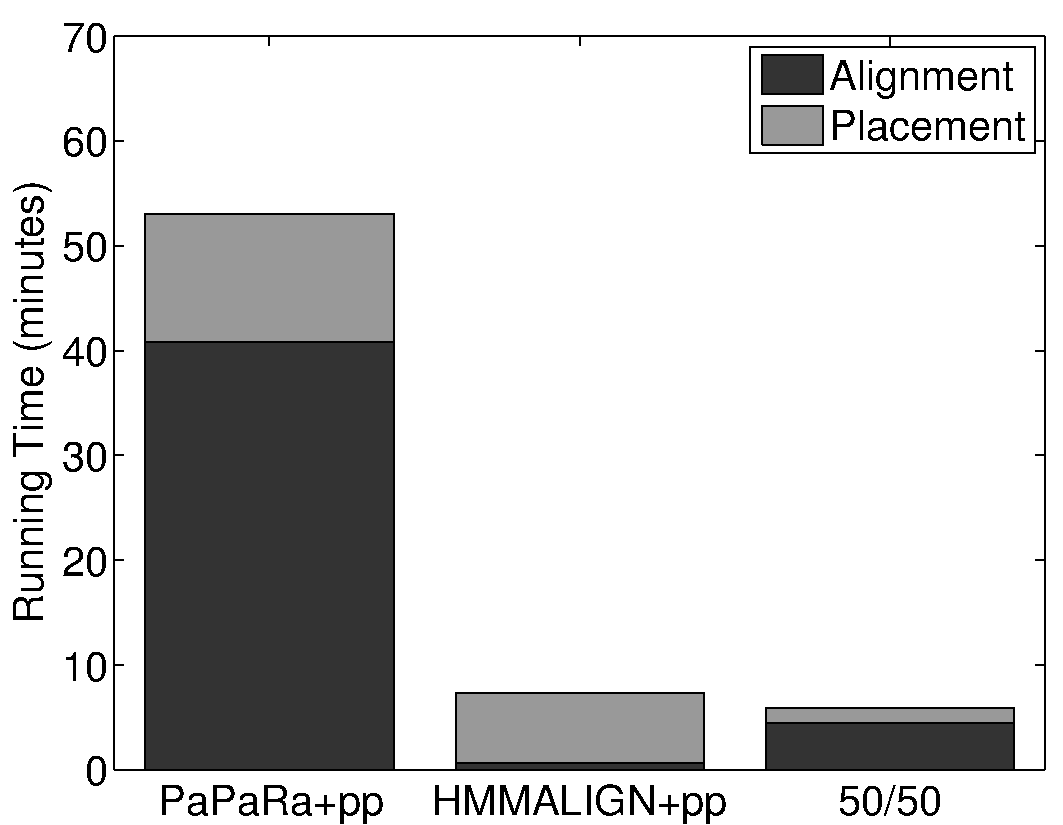
\includegraphics[width=0.35\textwidth]{sepp/M2-time-true}}
\\
%  \subfloat[\sate~backbone]
{\label{fig:sms}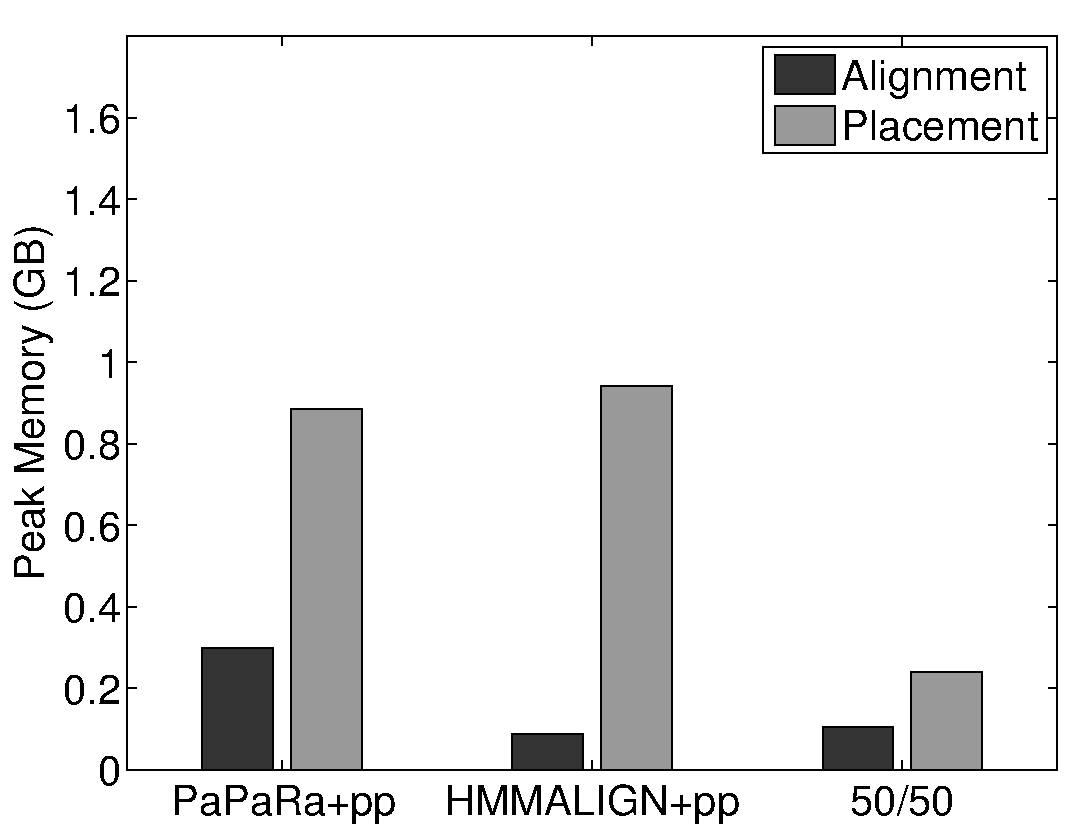
\includegraphics[width=0.35\textwidth]{sepp/M2-mem-sate}}
%  \subfloat[True backbone]
{\label{fig:smt}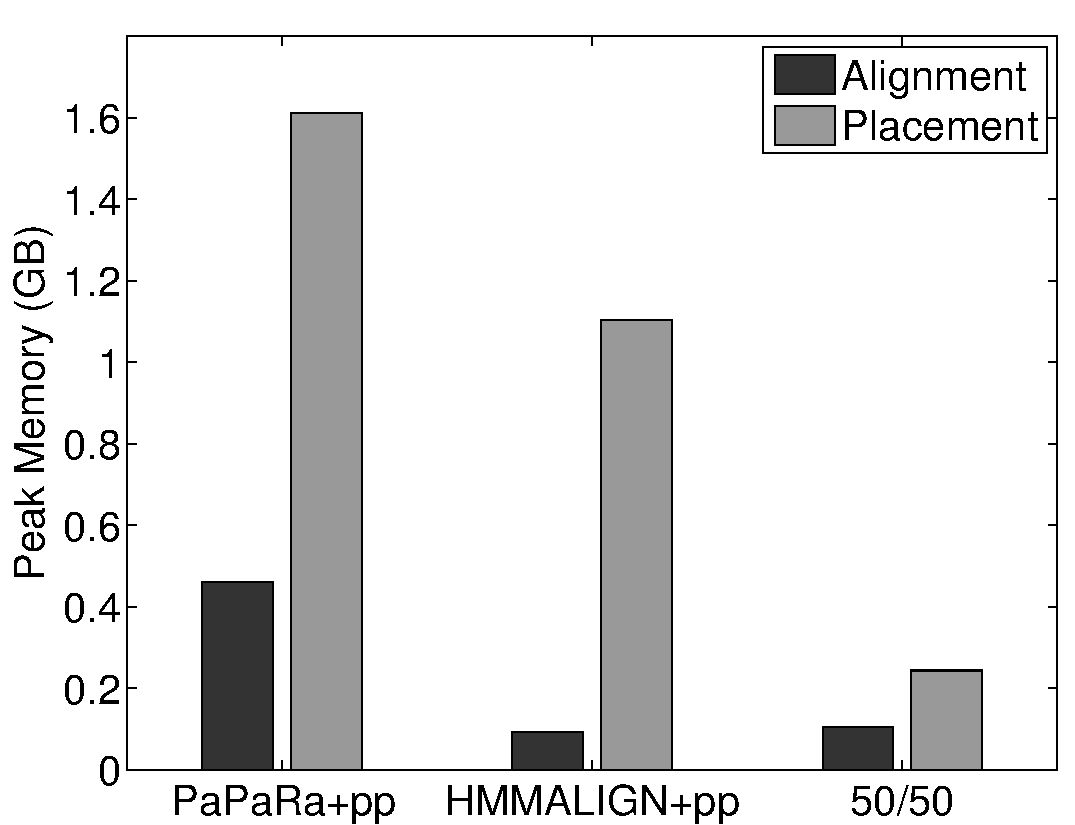
\includegraphics[width=0.35\textwidth]{sepp/M2-mem-true}}
\\
  \subfloat[\sate~backbone]
{\label{fig:ses}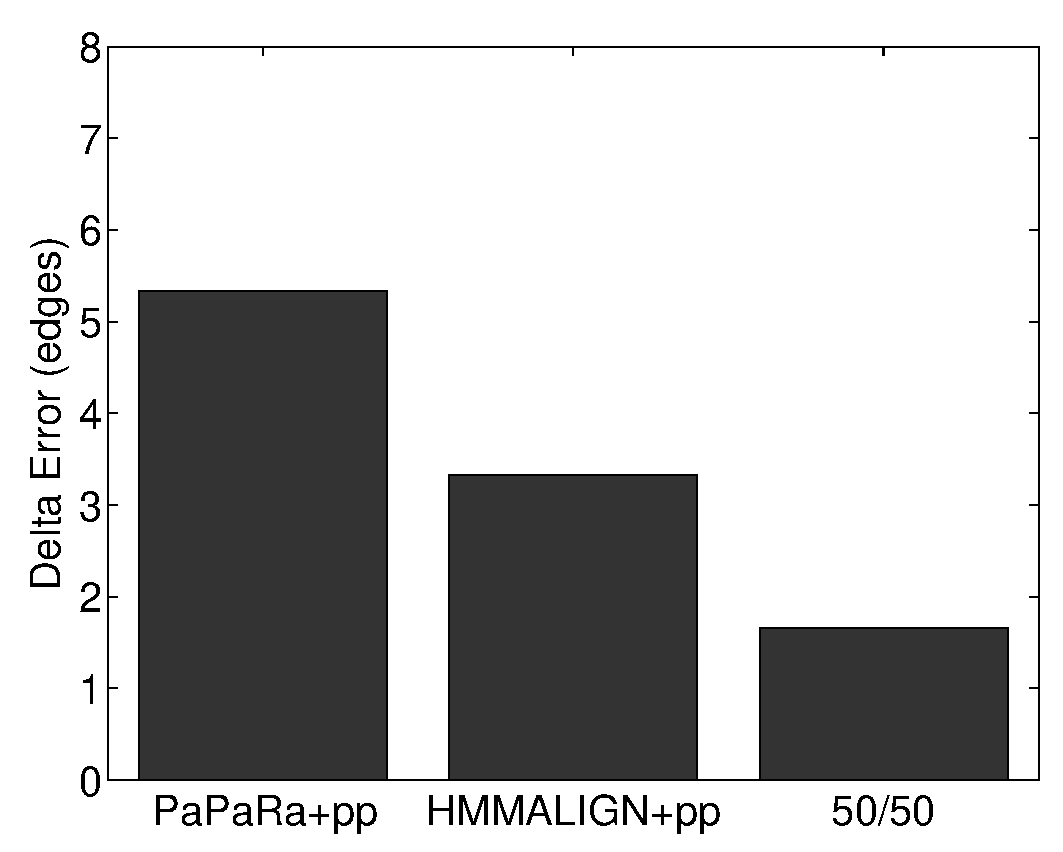
\includegraphics[width=0.35\textwidth]{sepp/M2-err-sate}}
  \subfloat[True backbone]
{\label{fig:set}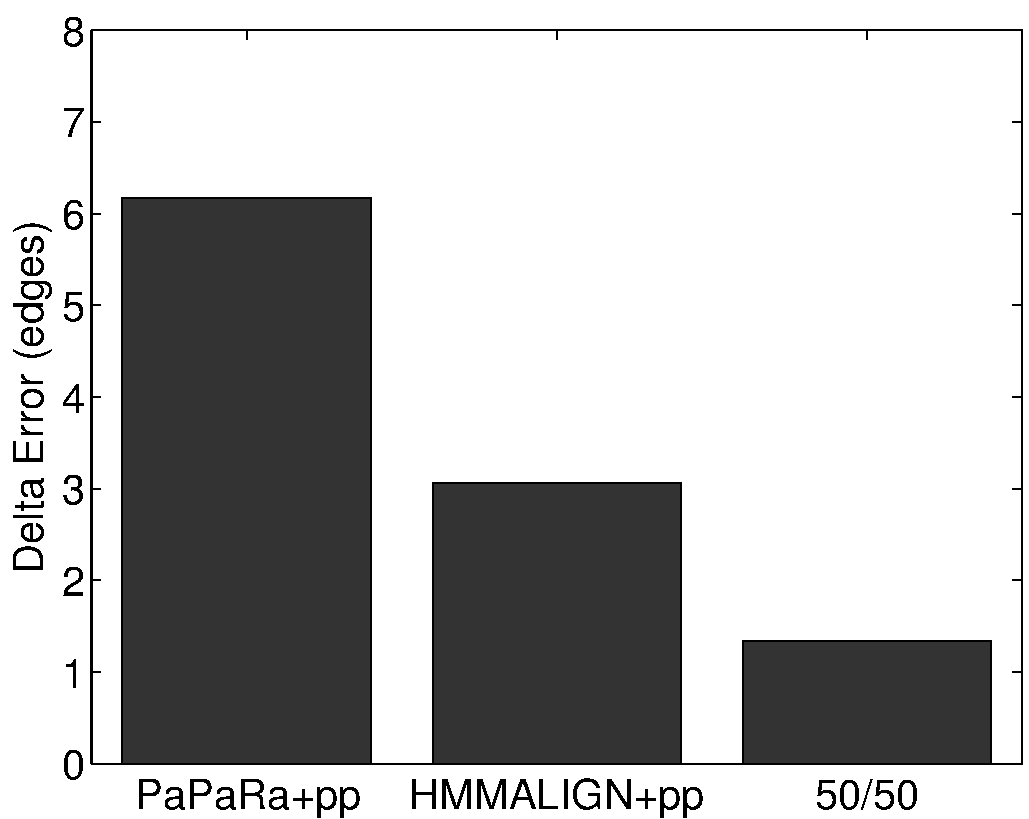
\includegraphics[width=0.35\textwidth]{sepp/M2-err-true}}
  \caption{Results on simulated datasets for model M2. I show running time (top), peak memory
usage (middle), and average number of additional missing branches per
query sequence (bottom).  Results for the SAT\'{e} backbone alignment and tree are on the
left, and results for the true backbone alignment and tree are on the
right.
The SAT\'{e} backbone tree has 12.1\% missing
branch rate and the backbone tree based upon the
true alignment has 0.09\% missing branch rate.
The number of additional missing branches shown (bottom) is the
increment above that amount.
}
  \label{fig:M2}
\end{figure}

\begin{figure}[htbp]
  \centering
%  \subfloat[Running time using \sate~backbone]
{\label{fig:bts}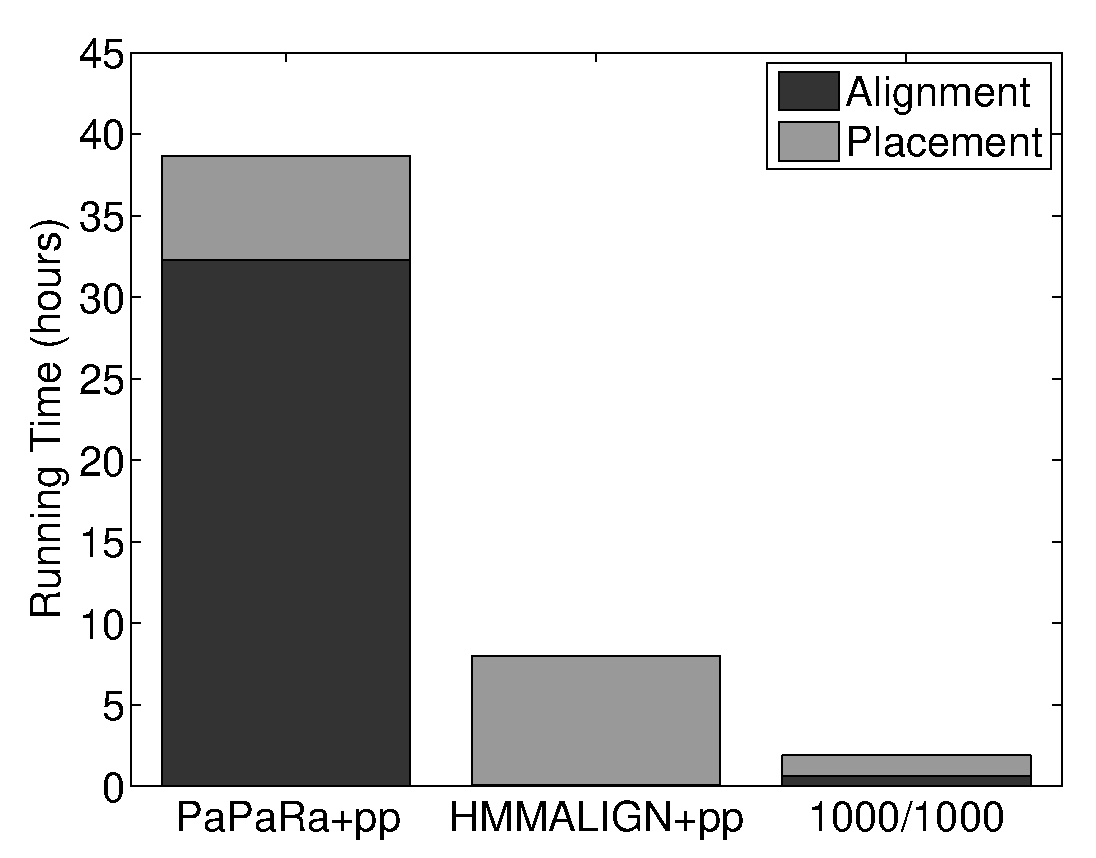
\includegraphics[width=0.35\textwidth]{sepp/bio-time-sate}}
%  \subfloat[Running time using curated backbone]
{\label{fig:btt}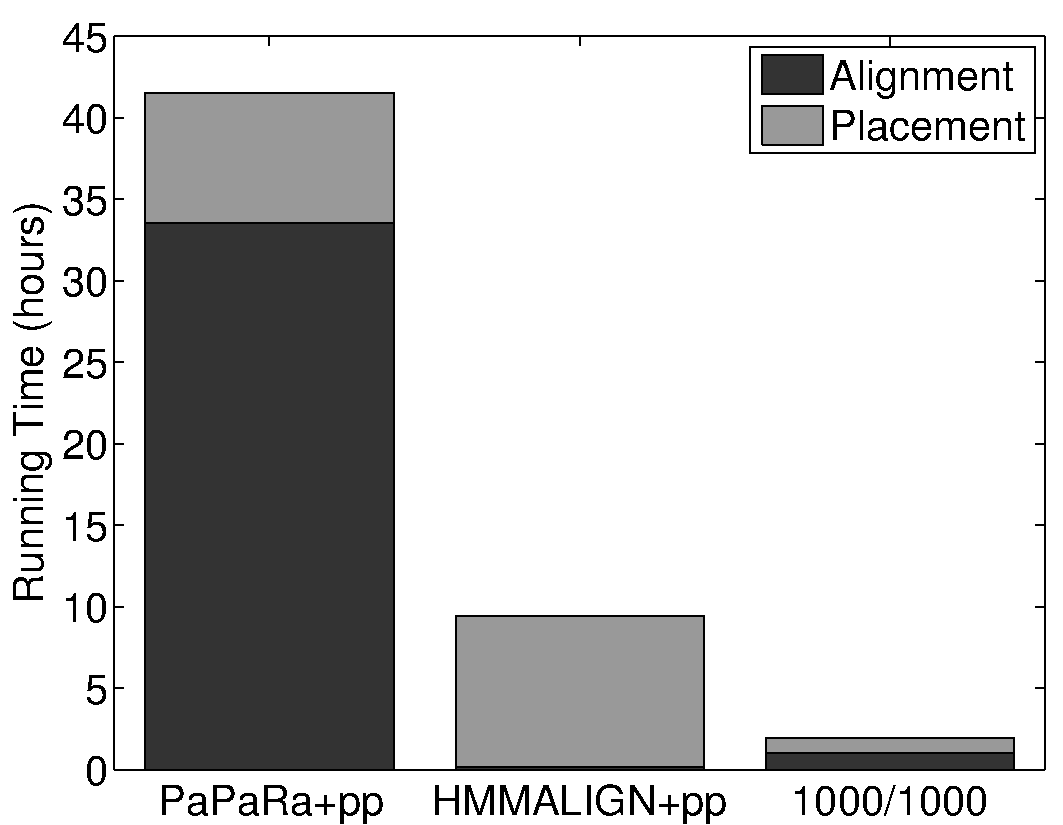
\includegraphics[width=0.35\textwidth]{sepp/bio-time-true}}
\\
%  \subfloat[Peak memory usage using \sate~backbone]
{\label{fig:bms}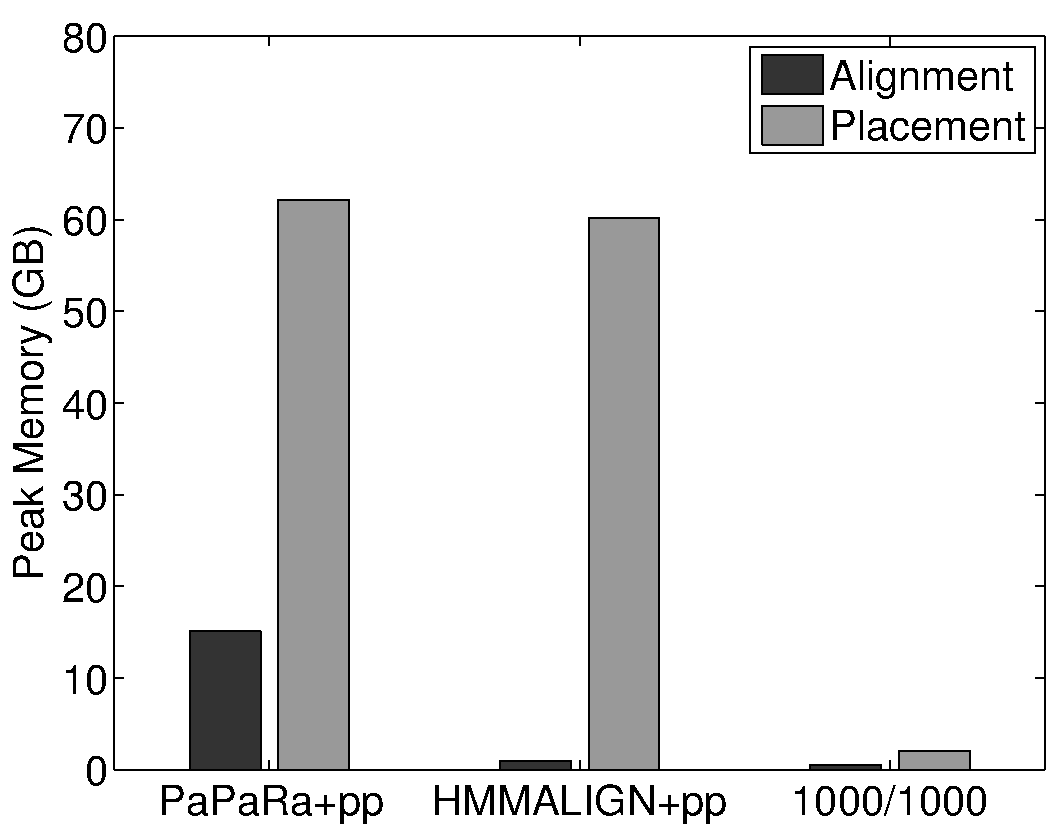
\includegraphics[width=0.35\textwidth]{sepp/bio-mem-sate}}
%  \subfloat[Peak memory usage using curated backbone]
{\label{fig:bmt}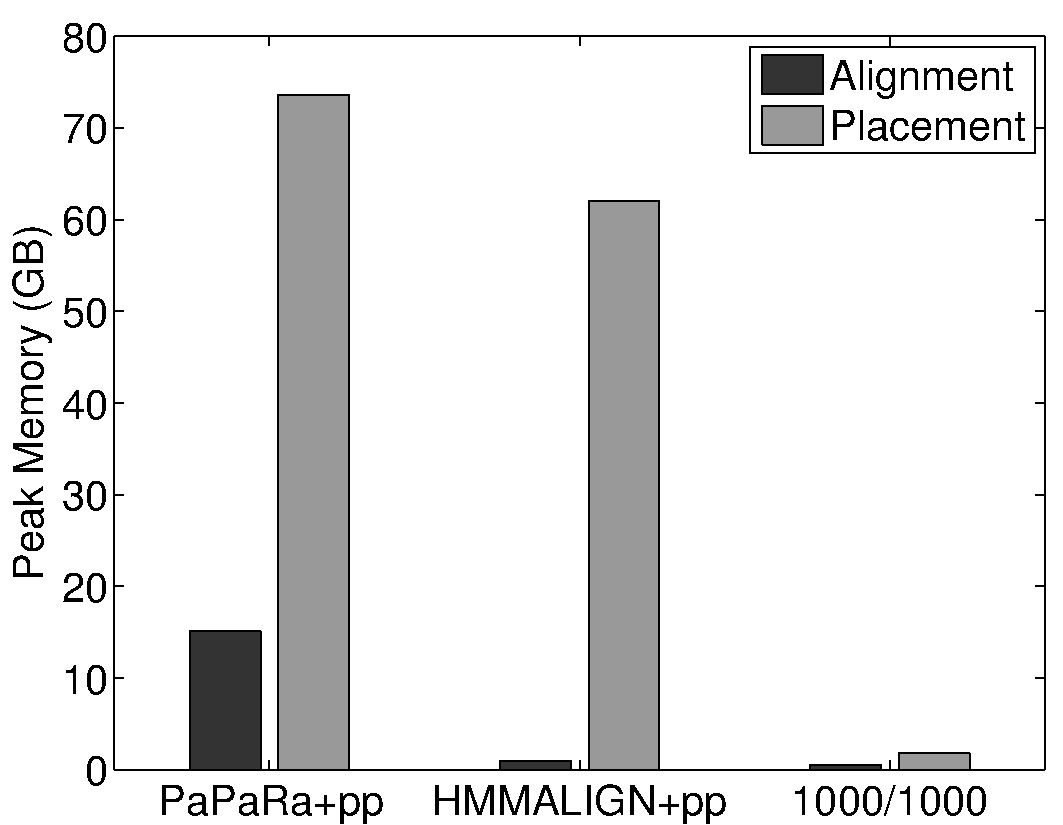
\includegraphics[width=0.35\textwidth]{sepp/bio-mem-true}}
\\
  \subfloat[\sate~backbone]
{\label{fig:bes}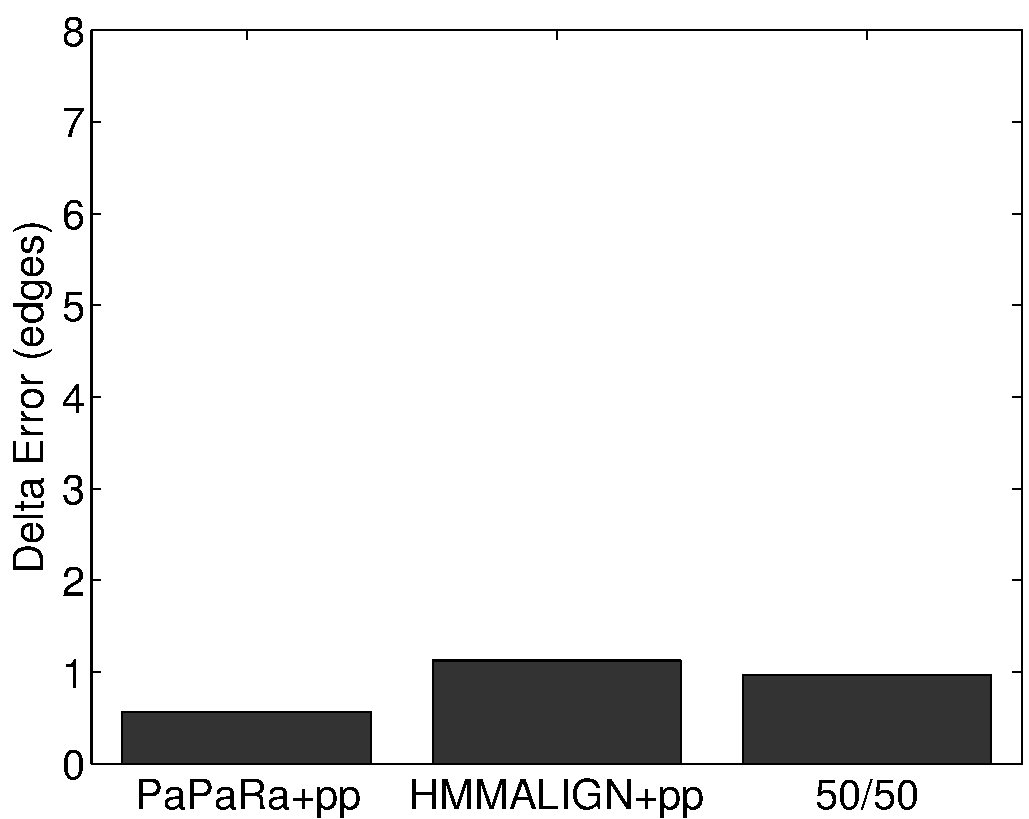
\includegraphics[width=0.35\textwidth]{sepp/bio-err-sate}}
  \subfloat[Curated backbone]
{\label{fig:bio}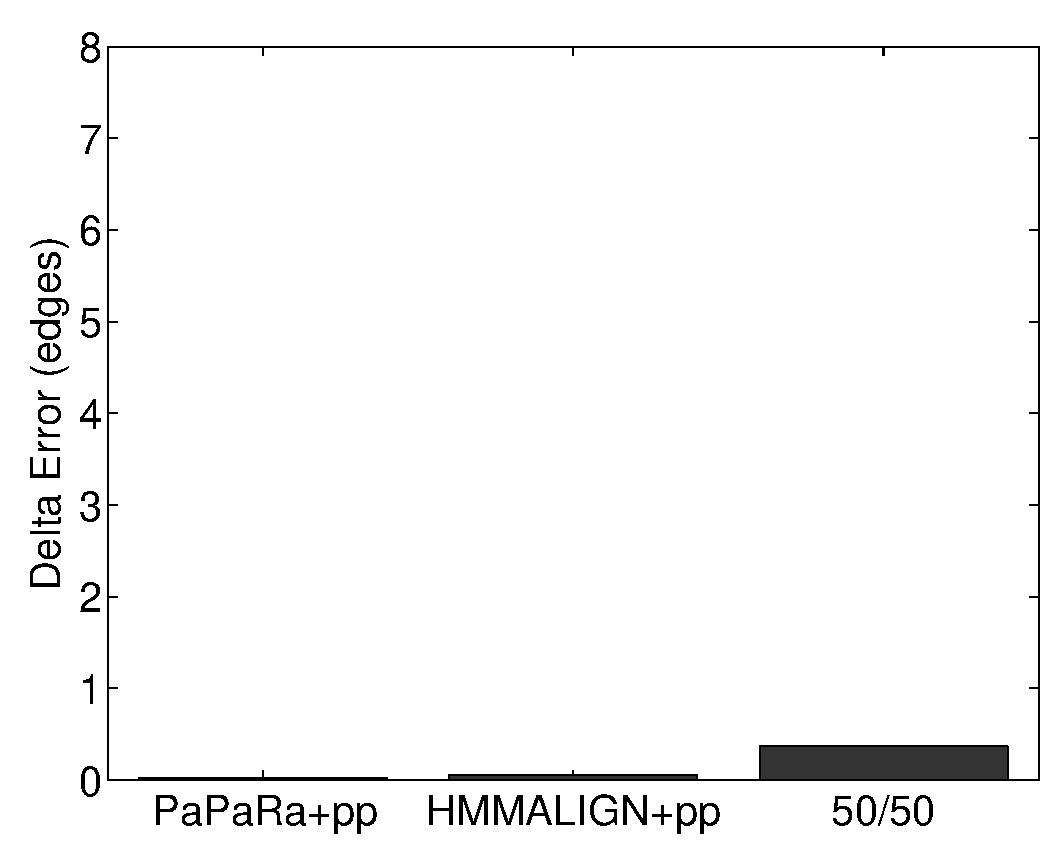
\includegraphics[width=0.35\textwidth]{sepp/bio-err-true}}
  \caption{Results on 16S.B.ALL. I show running time (top), peak memory
usage (middle), and average number of additional missing branches per
query sequence (bottom).  Results for the SAT\'{e} backbone alignment and tree are on the
left, and results for the curated backbone alignment and tree are on the
right. The SAT\'{e} missing branch rate is 7.64\%, and the
missing branch rate for the backbone tree defined by the
true alignment is 1.835\%.  The number of additional missing
branches shown (bottom) is the increment above that amount.}
  \label{fig:bio-all}
\end{figure}

\vspace{.1in}
\subsection{Results on simulated datasets}
The simulated datasets have backbone trees with 500 sequences
and fairly high rates of evolution, with M2 having the highest
rate and M4 having the lowest rate
(Table \ref{tab:datasets}).
Placement error rates were impacted by
the model, 
so that the missing branch rate
for all methods is higher on model M2 than on model M3,
and higher on model M3 than on model M4 (Table \ref{tab:reads-all}).
Not surprisingly, 
 absolute error rates are lower
with the true alignment and tree than with the SAT\'{e}
alignment and tree. 
These trends also held for
PaPaRa and SEPP.


\begin{table}[ht]
\begin{footnotesize}
 \caption{Mean delta-error for all query
sequences. I show the mean delta-error for each method on each model
condition for all the query sequences. 
Count refers to the number of query sequences processed and placed,
HMM refers to HMMALIGN+pplacer,
PPR refers to PaPaRa+pplacer, and SEPP refers to SEPP run in default mode.
}
 \label{tab:reads-all}
\begin{center}
{%
\begin{center}
\begin{tabular}{|l|llll|}
\hline
 & \mc{4}{c|}{ All reads}\\\hline
&bio.&M2   &M3   &M4   \\\hline
&\mc{4}{c|}{ \sate~Backbone}\\\hline
count&13819&99998&99999&99999\\
HMM&1.1&3.4&1.4&\textbf{0.3}\\
PPR&\textbf{0.6}&5.4&3.6&0.4\\
SEPP&1.0& \textbf{1.7}& \textbf{1} &0.4
\\\hline
&\mc{4}{c|}{ True or Curated Backbone}\\\hline
count&13818&99997&99999&99999\\
HMM&0.0&3.2&1.2&\textbf{0.0}\\
PPR&\textbf{0.0}&6.2&3.8&0.2\\
SEPP&0.4&\textbf{1.4}&\textbf{0.7}&0.1
\\\hline
\end{tabular}
\end{center}
}%
 \end{center}
\end{footnotesize}
\end{table}


\begin{table}[ht]
\begin{footnotesize}
 \caption{Mean delta-error for different categories of query
sequences. I show the mean delta-error for each method on each model
condition, as a function of the level of difficulty for the
query sequence, as estimated by HMMER. 
Count refers to the number of query sequences processed and placed,
HMM refers to HMMALIGN+pplacer,
PPR refers to PaPaRa+pplacer, and SEPP refers to SEPP run in default mode.
}
 \label{tab:reads-hard}

\begin{center}
{%
\begin{center}
\begin{tabular}{|l|llll|llll|}
\hline
  & \mc{4}{c|}{ Hard reads} & \mc{4}{c|}{Very hard reads}\\\hline
&bio.&M2   &M3   &M4   &bio.&M2   &M3   &M4\\\hline
&\mc{8}{c|}{ \sate~Backbone}\\\hline
count&104&79510&58924&3989&21&63613&40495&844\\
HMM&2.4&4.2&2.3&\textbf{0.7}&3.9&5.2 &3.2 &1.5\\
PPR&\textbf{0.8}&5.8&4.4&1.0& \textbf{0.9} &6.2 &4.9 &1.5\\
SEPP&2.4&\textbf{2.0}&\textbf{1.4}&0.8& 3.8& \textbf{2.4}& \textbf{1.8}& \textbf{1.0}
\\\hline
&\mc{8}{c|}{ True or Curated Backbone}\\\hline
count&104&79511&58924&3989&21&63614&40495&844\\
HMM&0.5&4.0&2.0&\textbf{0.2}&2.2&5.0&2.9&0.9\\
PPR&\textbf{0.1}&6.7&4.7&0.5&\textbf{0.0}&7.1&5.2&0.9\\
SEPP&1.1&\textbf{1.7}&\textbf{1.1}&0.4&1.5&\textbf{2.0}&\textbf{1.4}&\textbf{0.5}\\\hline
\end{tabular}
\end{center}
}%
 \end{center}
\end{footnotesize}
\end{table}

Figure \ref{fig:M2} and Table \ref{tab:reads-all} show results for
PaPaRa+pplacer, HMMALIGN+pplacer, and SEPP(50,50) (i.e.,
SEPP ran with the default
setting on this model of \ssa~= \ssp~= 50).
Note that SEPP(50,50)
has the lowest delta-error of the three
methods by far, 
followed by HMMALIGN+pplacer,
and then by PaPaRa+pplacer.
Furthermore, the differences are substantial.
The methods are clearly also distinguished by
running time and peak memory usage.
HMMALIGN+pplacer is the fastest, 
SEPP(50,50) is somewhat slower,
and PaPaRa uses much more time.
Both PaPaRa+pplacer
and HMMALIGN+pplacer use more memory than our method.

Results for M3 (see Table \ref{tab:reads-all})
are quite similar to M2, 
with
HMMALIGN+pplacer was much more accurate than PaPaRa+pplacer
and SEPP(50/50) produced more accurate placements
than HMMALIGN+pplacer.  However, the gap between SEPP(50,50) and
HMMALIGN+pplacer was reduced to only half an edge.
On M4 (see Table \ref{tab:reads-all}), however, the relative performance between SEPP(50,50) and HMMALIGN+pplacer depended on
the backbone tree. 
For the SAT\'{e} alignment/tree, SEPP(50,50) was
more accurate but slightly slower than HMMALIGN+pplacer.
For the true alignment/tree, 
HMMALIGN+pplacer was somewhat more accurate and took less
time. However, the difference in placement
accuracy between SEPP(50,50) and
HMMALIGN+pplacer
was extremely small - less than one-ninth of an edge for both
backbones.


\subsection{16S.B.ALL.}  
The datasets based upon  16S.B.ALL,
presented a different kind of challenge.
Each dataset had 13,820 query sequences
and a backbone tree with 13,822 sequences.
Thus, these datasets had much
larger backbone trees, but the backbone trees
and alignments reflected lower rates of evolution.

The default setting for SEPP on this dataset is \ssa~= \ssp~= 1000;
therefore, I ran SEPP(1000,1000) for both backbones.
Results on these datasets are shown in Figure \ref{fig:bio-all}.
Note that PaPaRa+pplacer provides a small
improvement in placement accuracy (slightly more than
half an edge)
in comparison to the other methods.  However, 
PaPaRa+pplacer is enormously computationally intensive, using
40 hours to analyze these data, 
much longer than either other method.
Also,  HMMALIGN+pplacer and PaPaRa+pplacer have
very large peak memory usage, near or above 60GB on both
backbone trees.  Thus, PaPaRa+pplacer is 
computationally extremely intensive, 
and possibly the improvement in placement accuracy is insufficient
given the additional running time costs.

A comparison of SEPP(1000,1000) to HMMALIGN+pplacer
shows that both have extremely good
placement accuracy, with delta-error approximately
one edge for both methods on the SAT\'{e}
backbone tree and well under half an edge on the
curated backbone tree.  
 HMMALIGN+pplacer
produces more accurate placements than our method
for the curated backbone and SEPP(1000,1000) produces
more accurate placements for the SAT\'{e} backbone,
but the differences between the
two methods are small in both cases (less
than a third of an edge).
The methods are, however, distinguished by their
computational requirements, as HMMALIGN+pplacer is
much slower (at least 4 times as much
time) and uses dramatically more memory (60GB as
compared to about 2GB).

\subsection{Comparing methods on query sequences of
different levels of difficulty}

Tables \ref{tab:reads-all} and \ref{tab:reads-hard} compares methods in 
terms of their placement accuracy as a function of 
the level of difficulty in placing the query sequence, as
predicted by HMMER (see the discussion in Section \ref{sec:studydesign}).
Note that error increases as the reads become more difficult,
as HMMER predicts.
I show that SEPP, run in default mode, performs very well
in general (as observed earlier) in comparison to
HMMALIGN+pplacer and PaPaRa+pplacer, but has a
particularly strong advantage on the hard and very hard reads.
Interestingly, PaPaRa+pplacer does well on hard
and very hard reads
for 16S.B.ALL but not on the simulated datasets.

\subsection{Summary}\label{sec:studydesign}
There are several observations we can make. First,
the methods I evaluated for
phylogenetic placement--PaPaRa+pplacer, HMMALIGN+pplacer,
and SEPP methods--often produce placements that are extremely accurate,
increasing the topological error over the input backbone tree
by at most an edge (often much less than an edge) on average.
Furthermore, while these methods do sometimes have 
differences in placement accuracy that go beyond an edge,
these differences are sometimes still
small enough to be relatively unimportant, compared 
to the computational cost
required to obtain the improved placement accuracy.

However, I did observe conditions  in which
the differences in placement accuracy were quite large, suggesting
that increased effort in placing query sequences correctly was
merited.  For example, 
I see big differences in
placement accuracy on model M2, resulting in
several edges improvement produced by SEPP(50,50)
over HMMALIGN+pplacer.
The  conditions under which
accuracy differences are substantial are characterized by large evolutionary
distances between some pairs of full-length sequences.
I conjecture that in such conditions, the HMMs produced by HMMER on
the full set of taxa may
not be sufficient to produce highly accurate alignments for the
query sequences, and will result in degraded placement accuracy.
The technique I introduce here avoids this problem by using HMMER to
produce HMMs
only on smaller, less diverse, subsets of the taxa.  As a result,
the HMMs may produce more accurate alignments to the query sequences,
and result in improved phylogenetic placement.

I note the interesting differences between
HMMALIGN+pplacer and PaPaRa+pplacer.  Only on the slowest evolving
dataset, 16S.B.ALL,  does
PaPaRa+pplacer produces more accurate placements than HMMALIGN+pplacer,
while PaPaRa+pplacer has substantially less accurate placements
for the faster evolving datasets.
This is consistent with the need to estimate transition state
matrices on each edge, an estimation that may only be highly
accurate under sufficiently low rates of evolution.

Furthermore, these methods differ dramatically with respect to
running time, with PaPaRa+pplacer much more computationally
intensive than HMMALIGN+pplacer and the default setting for
SEPP, thus suggesting that PaPaRa+pplacer is unlikely to
be useful in largescale metagenomic analyses.

The comparison between HMMALIGN+pplacer and SEPP is more
complex, because SEPP is parameterized by the two
algorithmic parameters \ssa~and \ssp. Here I see that some
very simple settings for these parameters (\ssa~= \ssp, both set to
about 10\% of the number of taxa in the backbone tree) produces very
fast results with generally very good accuracy, coming close to the
accuracy obtained by the best methods (or improving on them), but
in a fraction of the time.  
Other settings for the parameters can improve the placement accuracy but
require greater running time and memory usage.  


\section{Conclusion and future work}\label{sepp:conclusion}
In this chapter, I presented, SEPP, a general technique for boosting
the accuracy and/or speed of a phylogenetic placement method. 
I show in a simulation study its
performance when coupled with HMMALIGN+pplacer, and showed improvements
in placement accuracy and/or running time. Given the plans to analyze millions of reads, the speed-ups that SEPP provides could be essential to providing scalability for
phylogenetic placement methods.

I plan to explore other methods for estimating the extended alignment.
For example, improved accuracy might be obtained by
coupling SEPP with PaPaRa for those cases where
the backbone tree and alignment has slow evolutionary
rates to enable PaPaRa to produce highly accurate extended alignments.
Another potential method to examine is Mafft-profile~\cite{Katoh2012}.
Mafft-profile takes in a backbone alignment and a sequence of query sequences and aligns each query sequence to the backbone alignment.  Mafft-profile can be run under an accurate setting (``addfragments'' and ``L-INS-I''), however,
the most accurate setting can only be run on a backbone alignment of 1000 sequences.  More accurate placements may be obtained if Mafft-profile is used within SEPP, using the decomposition technique to allow Mafft-profile to scale to larger datasets.

Based on the placement of the query sequence, the evolutionary relationship between the query sequence and the sequences in the backbone alignment can be inferred.  Thus, SEPP can be used to taxonomically identify unknown reads based upon the placement of the sequence in the backbone tree.  In Chapter~\ref{tipp_chapter}, I will show how SEPP fares toward taxonomic indentification and how SEPP can be modified to obtain improved classification accuracy.  Finally, the one of the outputs of SEPP is an alignment of the query sequences to the backbone alignment.  For phylogenetic placement, the individual alignment of each query sequence to the backbone alignment is used to locate the placement, and thus, the query sequences have no impact on each other, both in alignment and placement.  This does not necessarily have to be the case.  In Chapter~\ref{upp_chapter}, I will show how SEPP can be modified for ultra-large alignments and how estimating trees on the entire alignment outputted from SEPP, including all the backbone sequences and query sequences, can result in accurate phylogeny estimation.
